% PTE Core 模考 1B —— 总整理卷（听·说·读·写 合订，自包含）
% 编译: xelatex 本文件.tex（跑两遍，目录页码才对）；依赖同目录 img/。
\documentclass[11pt]{article}

% --------- 样式（原 ptestyle.sty，已内联）---------
% ============================================================
%  ptestyle.sty  —  PTE 模考错题整理卷 共享样式
%  编译引擎: XeLaTeX  (中英混排, 需要 Noto CJK 字体)
% ============================================================

\usepackage[a4paper,margin=2cm,headsep=4mm]{geometry}
\usepackage{fontspec}
\usepackage{xeCJK}
\usepackage[table]{xcolor}
\usepackage[normalem]{ulem}        % \sout 删除线
\usepackage{tabularx}
\usepackage{array}
\usepackage{ragged2e}
\usepackage{enumitem}
\usepackage[most]{tcolorbox}
\usepackage{fancyhdr}
\usepackage{graphicx}
\usepackage{pifont}                % \ding{51}=✓ \ding{55}=✗（阅读对错标注）
\usepackage{needspace}
\usepackage{tikz}

% ---------- 字体 ----------
\setmainfont{TeX Gyre Heros}            % 拉丁: Helvetica 风格(纤细清晰)
\setCJKmainfont{Noto Sans CJK SC}
\setCJKsansfont{Noto Sans CJK SC}
\newfontfamily\cjkserif{Noto Serif CJK SC}
\linespread{1.18}
\setlength{\parindent}{0pt}
\setlength{\parskip}{4pt}

% ---------- 配色 ----------
\definecolor{cWrong}{HTML}{D32F2F}     % 红  = 修改 / 错误
\definecolor{cFix}{HTML}{1B7F3B}       % 绿  = 正确建议
\definecolor{cDelete}{HTML}{1565C0}    % 蓝  = 删除
\definecolor{cInsert}{HTML}{7B1FA2}    % 紫  = 插入
\definecolor{cPartial}{HTML}{E07B00}   % 橙  = 部分得分
\definecolor{cNote}{HTML}{0277BD}      % 蓝  = 注解
\definecolor{cAccent}{HTML}{16A085}    % 主题青绿(平台主色)
\definecolor{cWrongBg}{HTML}{FBE0E0}
\definecolor{cDelBg}{HTML}{DCE8FB}
\definecolor{cInsBg}{HTML}{EEE0F5}
\definecolor{cHead}{HTML}{20303A}
\definecolor{cGrayBox}{HTML}{F4F6F7}
\definecolor{cModelBg}{HTML}{EAF7EF}
\definecolor{cYouBg}{HTML}{FFF7F5}
\definecolor{cNoteBg}{HTML}{EAF3FA}
\definecolor{cRule}{HTML}{D7DEE2}

% ---------- 行内批改宏 (复刻平台标注) ----------
% \fix{原词}{正确}  红色删除线 + 绿色上标改正  (修改/拼写/空格)
\newcommand{\fix}[2]{%
  \colorbox{cWrongBg}{\textcolor{cWrong}{\sout{#1}}}%
  \,\textsuperscript{\textcolor{cFix}{\footnotesize #2}}}
% \del{原词}  蓝色删除线  (应删除)
\newcommand{\del}[1]{%
  \colorbox{cDelBg}{\textcolor{cDelete}{\sout{#1}}}%
  \,\textsuperscript{\textcolor{cDelete}{\footnotesize 删}}}
% \ins{词}  紫色下划线  (应插入)
\newcommand{\ins}[1]{%
  \textsuperscript{\textcolor{cInsert}{\footnotesize $\wedge$}}%
  \colorbox{cInsBg}{\textcolor{cInsert}{#1}}}
% \miss{词}  灰色删除线  (口语漏读 / 未作答)
\newcommand{\miss}[1]{\textcolor{gray}{\sout{#1}}}
% \add{原词}{改正}  橙色波浪线 + "补"标签  (平台漏标、本卷补标的错误)
\definecolor{cAdd}{HTML}{E65100}
\newcommand{\add}[2]{%
  \textcolor{cAdd}{\uwave{#1}}%
  \,\textsuperscript{\textcolor{cAdd}{\footnotesize 补：#2}}}
% 高亮(口语发音): 好/中/差
\newcommand{\spk}[2]{\textcolor{#1}{#2}}

% ---------- 评分单元格着色 ----------
\newcommand{\sfull}[1]{\textcolor{cFix}{\bfseries #1}}     % 满分
\newcommand{\spart}[1]{\textcolor{cPartial}{\bfseries #1}} % 部分
\newcommand{\szero}[1]{\textcolor{cWrong}{\bfseries #1}}   % 零/低分

% ---------- 分数小标签 ----------
\newtcbox{\chip}[1][cAccent]{on line, boxsep=2pt, left=4pt, right=4pt, top=1pt,
  bottom=1pt, arc=3pt, colback=#1, colframe=#1, coltext=white, nobeforeafter,
  fontupper=\bfseries\footnotesize}

% ---------- 题块小标题 ----------
\newcommand{\ptesub}[1]{%
  \par\needspace{2\baselineskip}\smallskip
  {\color{cAccent}\rule[-0.2ex]{3pt}{1.05em}}\hspace{6pt}%
  {\bfseries\color{cHead}#1}\par\nopagebreak\smallskip}

% ---------- 题块外框 ----------
% \begin{qblock}{标号·题型}{右上信息(得分/用时)} ... \end{qblock}
\newtcolorbox{qblock}[2]{
  breakable, enhanced, arc=2.5pt,
  colback=white, colframe=cRule, boxrule=0.6pt,
  left=11pt, right=11pt, top=8pt, bottom=10pt,
  toptitle=3pt, bottomtitle=3pt, lefttitle=11pt, righttitle=11pt,
  colbacktitle=cHead, coltitle=white, fonttitle=\bfseries,
  title={#1\hfill\normalfont\bfseries\small #2}}

% ---------- 文本块: 题干 / 范文 / 你的作答 / 建议 ----------
\newtcolorbox{promptbox}{enhanced, breakable, colback=cGrayBox, colframe=cGrayBox,
  arc=2pt, left=8pt, right=8pt, top=6pt, bottom=6pt, boxrule=0pt}
\newtcolorbox{modelbox}{enhanced, breakable, colback=cModelBg, colframe=cModelBg,
  borderline west={3pt}{0pt}{cFix}, arc=1pt, left=8pt, right=8pt, top=6pt, bottom=6pt, boxrule=0pt}
\newtcolorbox{youbox}{enhanced, breakable, colback=cYouBg, colframe=cYouBg,
  borderline west={3pt}{0pt}{cWrong}, arc=1pt, left=8pt, right=8pt, top=6pt, bottom=6pt, boxrule=0pt}
\newtcolorbox{notebox}{enhanced, breakable, colback=cNoteBg, colframe=cNoteBg,
  borderline west={3pt}{0pt}{cNote}, arc=1pt, left=8pt, right=8pt, top=6pt, bottom=6pt, boxrule=0pt}

% ---------- 评分表 ----------
% 用法见正文; 这里给表头宏
\newcommand{\scorehead}{%
  \rowcolors{2}{cGrayBox}{white}
  \arrayrulecolor{cRule}}

% ---------- 章节大标题 ----------
\newcommand{\ptesection}[3]{% #1=中文名 #2=英文名 #3=该项分数
  \addcontentsline{toc}{section}{#1}%
  \needspace{6\baselineskip}
  \begin{tcolorbox}[enhanced, colback=cAccent, colframe=cAccent, sharp corners,
     left=14pt, right=14pt, top=10pt, bottom=10pt, boxrule=0pt]
    {\fontsize{20}{24}\selectfont\bfseries\color{white} #1\ \ }%
    {\large\color{white!85} #2}\hfill
    {\large\color{white}本项得分\ \ }{\fontsize{22}{24}\selectfont\bfseries\color{white} #3}%
    \ {\color{white!85}/ 90}
  \end{tcolorbox}}

% ---------- 题型小节分隔 (口语 RA/RS/DI/RTS/ASQ 等) ----------
\newcommand{\ptetask}[2]{%
  \addcontentsline{toc}{subsection}{#1\ #2}%
  \needspace{4\baselineskip}\medskip
  \begin{tcolorbox}[enhanced, colback=cHead, colframe=cHead, sharp corners,
     left=12pt, right=12pt, top=5pt, bottom=5pt, boxrule=0pt]
    {\large\bfseries\color{white} #1}\ \ {\color{white!80} #2}
  \end{tcolorbox}\smallskip}

% ---------- 口语 AI 语音识别着色 (复刻平台: 优/良/差 + 停顿) ----------
\definecolor{cSpkGood}{HTML}{2E9E5B}   % 优 绿
\definecolor{cSpkOk}{HTML}{C77F00}     % 良 黄/琥珀
\definecolor{cSpkBad}{HTML}{E0352B}    % 差 红
\newcommand{\sg}[1]{\textcolor{cSpkGood}{#1}}   % 优
\newcommand{\sy}[1]{\textcolor{cSpkOk}{#1}}     % 良
\newcommand{\sr}[1]{\textcolor{cSpkBad}{#1}}    % 差
\newcommand{\smiss}[1]{\textcolor{cSpkBad}{\sout{#1}}}  % 漏读 (红删除线)
\newcommand{\pse}{{\color{gray}\,/\,}}          % 停顿
\newcommand{\asrlegend}{{\footnotesize\color{gray}AI 语音识别\quad
  {\color{cSpkGood}\textbullet}\,优\ \ {\color{cSpkOk}\textbullet}\,良\ \
  {\color{cSpkBad}\textbullet}\,差\ \ {\color{gray}/}\,停顿\ \
  {\color{cSpkBad}\sout{词}}\,漏读}}
\newtcolorbox{asrbox}{enhanced, breakable, colback=white, colframe=cRule,
  boxrule=0.6pt, arc=1pt, left=8pt, right=8pt, top=6pt, bottom=6pt}

% ---------- 中文翻译行 ----------
\newcommand{\zh}[1]{{\footnotesize\textcolor{cNote}{\textbf{译}}\ \textcolor{gray}{#1}}}

% ---------- 阅读填空 / 选择 对错标注 ----------
\newcommand{\rok}[1]{{\color{cFix}\ding{51}\,#1}}                 % 选对(绿勾 + 词)
\newcommand{\rno}[2]{{\color{cWrong}\ding{55}\,\sout{#1}}\,{\footnotesize\color{cFix}(答案:\,#2)}}  % 选错: 你的(红删) + (答案:正确)
\newcommand{\rblank}[1]{{\color{cFix}\underline{\,#1\,}}}         % 直接给空的正确答案(无你的作答时)

% ---------- 听力专用 ----------
\newcommand{\hiw}[2]{{\color{cWrong}\uline{#1}}\,{\footnotesize\color{cFix}(听:#2)}} % HIW: 屏幕错词(红下划线)+ 实际读音
\newcommand{\lhit}[1]{{\color{cFix}#1}}                           % WFD: 命中的词(绿)
\newcommand{\lmiss}[1]{{\color{cWrong}\sout{#1}}}                 % WFD: 多余/错误的词(红删)

% ---------- 颜色图例 ----------
\newcommand{\ptelegend}{%
  \begin{tcolorbox}[enhanced, colback=cGrayBox, colframe=cRule, boxrule=0.5pt,
    arc=2pt, left=10pt, right=10pt, top=6pt, bottom=6pt]
  {\bfseries\color{cHead}颜色说明\quad}
  \fix{改}{正}~修改/拼写\quad
  \del{删}~应删除\quad
  \ins{插}~应插入\quad
  \add{补}{改正}~平台漏标(本卷补标)\quad
  {\color{cFix}\rule{1em}{0.6em}}~范文/正确\quad
  {\color{cNote}\rule{1em}{0.6em}}~AI 建议
  \end{tcolorbox}}

% ---------- 页眉页脚 ----------
\pagestyle{fancy}
\fancyhf{}
\renewcommand{\headrulewidth}{0.4pt}
\renewcommand{\footrulewidth}{0pt}
\fancyhead[L]{\footnotesize\color{cHead}\bfseries PTE Core 模考 1B}
\fancyhead[R]{\footnotesize\color{gray} 错题与详解整理卷}
\fancyfoot[C]{\footnotesize\color{gray}\thepage}
\renewcommand{\contentsname}{目录\quad Contents}

\begin{document}

% --------- 封面（原 cover.tex）---------
% ---------- 封面 / 成绩总览 ----------
\definecolor{mListen}{HTML}{1F3A5F}
\definecolor{mRead}{HTML}{C2D70B}
\definecolor{mSpeak}{HTML}{4D4D4D}
\definecolor{mWrite}{HTML}{A01B7D}

\begin{titlepage}
\thispagestyle{empty}
\centering
\vspace*{1.4cm}

{\fontsize{30}{36}\selectfont\bfseries\color{cHead} PTE Core 模考 1B}\\[4mm]
{\fontsize{17}{20}\selectfont\color{cAccent}\bfseries 错题与详解 · 整理卷}\\[3mm]
{\color{gray} APEUni / 猩际 PTE 模考　·　提交时间 2026-06-21 12:36}\\[1.2cm]

% ---- 总分 ----
\begin{tcolorbox}[width=0.62\textwidth, halign=center, enhanced,
  colback=cAccent, colframe=cAccent, arc=6pt, boxrule=0pt, top=10pt, bottom=10pt]
  {\color{white}\large 总分 Overall}\\[2pt]
  {\fontsize{46}{50}\selectfont\bfseries\color{white} 40}
\end{tcolorbox}

\vspace{1.0cm}

% ---- 四项分数条形图 ----
\begin{tcolorbox}[width=0.84\textwidth, enhanced, colback=white, colframe=cRule,
  boxrule=0.8pt, arc=4pt, left=18pt, right=18pt, top=14pt, bottom=14pt]
\setlength{\tabcolsep}{6pt}\renewcommand{\arraystretch}{1.7}
\sffamily
\begin{tabular}{@{}r@{\hskip 8pt}l@{\hskip 10pt}l@{}}
 \bfseries Listening 听力 & {\color{mListen}\rule{3.67cm}{0.42cm}} & {\bfseries\large 33}\\
 \bfseries Reading 阅读   & {\color{mRead}\rule{4.67cm}{0.42cm}}   & {\bfseries\large 42}\\
 \bfseries Speaking 口语  & {\color{mSpeak}\rule{3.22cm}{0.42cm}}  & {\bfseries\large 29}\\
 \bfseries Writing 写作   & {\color{mWrite}\rule{6.33cm}{0.42cm}}  & {\bfseries\large 57}\\
\end{tabular}\\[2mm]
{\footnotesize\color{gray} 满分 90　|　刻度: 条长 = 得分 / 90}
\end{tcolorbox}

\vfill
\begin{flushleft}\small\color{gray}
\textbf{说明:}本卷由本次模考的题目与"详解"截图逐题誊写、重新排版而成,完整保留每道题的
\emph{题干 / 原文、范文、你的作答、逐项评分、彩色批改与 AI 中文建议}。\\
所有错误按平台标注用颜色标出(见下方图例)。原始"详解"PDF 不可复制、仅截图,本卷内容均为人工对照誊录,若与原图有出入以原图为准。
\end{flushleft}
\vspace{4mm}
\ptelegend
\end{titlepage}

% --------- 目录 + 本卷概览 ---------
\clearpage
\tableofcontents
\bigskip

{\large\bfseries\color{cAccent}本卷概览}\par\smallskip
{\small
\begin{tabularx}{\linewidth}{@{}l c >{\RaggedRight\arraybackslash}X r@{}}
\rowcolor{cHead}\textcolor{white}{\bfseries 部分} & \textcolor{white}{\bfseries 题量} & \textcolor{white}{\bfseries 题型构成} & \textcolor{white}{\bfseries 本项得分}\\
听力 Listening & 15 & SST · MCM-L · FIB-L\,$\times$3 · MCS-L · SMW\,$\times$2 · HIW\,$\times$3 · WFD\,$\times$4 & 33 / 90\\
口语 Speaking & 30 & RA\,$\times$7 · RS\,$\times$11 · DI\,$\times$3 · RTS\,$\times$3 · ASQ\,$\times$6 & 29 / 90\\
阅读 Reading & 16 & FIB\,$\times$5 · MCM\,$\times$2 · RO\,$\times$2 · FIB(R)\,$\times$5 · MCS\,$\times$2 & 42 / 90\\
写作 Writing & \phantom{0}4 & SWT\,$\times$2 · WE\,$\times$2 & 57 / 90\\
\end{tabularx}}
\par\smallskip
{\footnotesize\color{gray}总分 40（听力 33 / 阅读 42 / 口语 29 / 写作 57）。颜色与标注沿用各部分；本合订本顺序为「听·说·读·写」。}

\clearpage
% --------- 四部分正文 ---------
% ===== sec_listening_body.tex =====
% ===================== 听力 Listening =====================
\ptesection{听力}{Listening · SST + MCM + FIB + MCS + SMW + HIW + WFD}{33}

\vspace{1mm}
{\small\color{gray} 依据「听力1 / 听力2」逐题誊录，并用「听力0 / 听力详解1」补全 SST 评分明细、用长截图补全 PDF 中被悬浮按钮遮挡处。
本套听力共 \textbf{15} 题：SST 概述口语$\times$1、MCM-L 多选$\times$1、FIB-L 听力填空$\times$3、MCS-L 单选$\times$1、SMW 选词$\times$2、HIW 找错词$\times$3、WFD 听写$\times$4。}
\vspace{1mm}

\begin{notebox}
{\footnotesize 标注沿用阅读：{\color{cFix}\ding{51}\,绿=对/命中}；{\color{cWrong}\ding{55}\,红删=错}，其后 {\color{cFix}(答案/听: 正确)}。
\textbf{HIW}（找错词）：屏幕上与录音不符的词用 {\color{cWrong}\uline{红下划线}} 标出（即应点选的"错词"），括注实际读音。
\textbf{WFD}（听写）：{\color{cFix}绿}=命中词，{\color{cWrong}\sout{红删}}=多写/听错的词。}
\end{notebox}

% =================== Q1 ===================
\begin{qblock}{Q1\quad SST (C) \#21\ \ Role of Education}{概述口语 Summarize Spoken Text · 评分 \textcolor{cAccent}{\bfseries 7 / 10}}
\ptesub{录音原文 Transcript}
\begin{promptbox}
Education stands as a powerful tool in bridging social inequalities, serving as a catalyst for change in a world riddled with disparities. Its role in shaping a more equitable society is paramount, as it offers the key to unlocking potential and leveling the playing field. However, the journey towards educational equity is fraught with challenges. In many parts of the world, access to quality education is unevenly distributed, often influenced by factors such as socioeconomic status, race, and gender. This disparity perpetuates a cycle of inequality, where underprivileged groups remain marginalized. The digital divide, exacerbated by the recent global pandemic, has further highlighted these disparities. Students in remote or impoverished areas, lacking access to technology and the internet, find themselves at a significant disadvantage. However, there is hope. Initiatives aimed at providing equitable access to education, such as scholarship programs, community schools, and digital learning platforms, have shown promise. They not only offer access to knowledge but also foster critical thinking and problem-solving skills, empowering individuals to rise above their circumstances.
\end{promptbox}
\zh{教育是弥合社会不平等的有力工具，在一个充满差距的世界里充当变革的催化剂。它在塑造更公平社会中的作用至关重要，因为它提供了释放潜能、创造公平竞争环境的钥匙。然而，通往教育公平的道路充满挑战。在世界许多地方，优质教育的获取分布不均，常受社会经济地位、种族和性别等因素影响。这种差距使不平等的循环延续，弱势群体始终被边缘化。近期的全球疫情加剧了数字鸿沟，进一步凸显了这些差距：身处偏远或贫困地区、缺乏技术与网络的学生处于明显劣势。然而，希望仍在。旨在提供公平教育机会的举措——如奖学金项目、社区学校和数字学习平台——已显现成效；它们不仅提供获取知识的途径，还培养批判性思维和解决问题的能力，使个人能够超越自身处境。}
\ptesub{你的概述 Your Summary}
\begin{promptbox}
The education is important. {\color{cAccent}\uline{The society}} has some {\color{cAccent}\uline{journal}} challenges. The influence {\color{cAccent}\uline{contain}} society and gender. The community has some critical skills.
\end{promptbox}
{\footnotesize\color{gray}（AI 标注待改：The/The society 多余冠词；journal 疑为听错词（general?）；contain → contains 主谓一致。）}
\ptesub{AI 评分明细（本题 10 分，得 \textcolor{cAccent}{\bfseries 7} 分）}
\begin{notebox}\small
\begin{tabular}{@{}lcl@{}}
Content（内容）& \textbf{2 / 2} & 内容很棒\\
Form（字数形式）& \textbf{2 / 2} & 很棒，这是必拿分数\\
Grammar（语法）& \textcolor{cWrong}{\bfseries 0 / 2} & SST 中占分比重、却很容易提高；丢分较多，建议针对性练习\\
Spelling（拼写）& \textbf{2 / 2} & 拼写很棒，再接再厉\\
Vocabulary（词汇）& \textbf{1 / 2} & PTE 不要求难词，但需用词恰当\\
\end{tabular}
\end{notebox}
\end{qblock}

% =================== Q2 ===================
\begin{qblock}{Q2\quad MCM-L \#20\ \ Re-adjusting to Life}{多选 Multiple Answers · 评分 \textcolor{cAccent}{\bfseries 1 / 2}}
\ptesub{录音原文 Transcript}
\begin{promptbox}
Re-adjusting to life in your own country after living abroad for some time is a little like recovering from jet-lag after a long flight across several time zones. It takes time. And research indicates that after nine years living in a foreign country you never really do re-adjust. Of course, things have changed: governments have come and gone, what you knew as countryside has become a suburb, new technologies have changed the way people go about their daily lives, and so on. These changes may well have been taking place in your adopted country, but they were happening while you were there, so you could adapt as you went along. Those are not the main difficulties, however. It is in the smaller, everyday things that you might experience what is known as culture shock, although it's not really a shock, but puzzling all the same. For example, the precise way to behave at a supermarket checkout may have changed. And in ordinary conversation, the frames of reference have changed, and quite often you find that you don't really know what people are talking about, even though they are speaking your native tongue.
\end{promptbox}
\zh{在国外生活一段时间后回到自己国家重新适应，有点像长途跨时区飞行后倒时差——需要时间。研究表明，在国外生活九年后，你其实永远无法真正重新适应。当然，一切都变了：政府换了一届又一届，你记忆中的乡村变成了郊区，新技术改变了人们的日常生活方式，等等。这些变化在你侨居的国家或许也在发生，但那是在你在场时发生的，所以你能边走边适应。然而，那些并不是主要困难。真正的困难在于更小的日常琐事——你可能经历所谓“文化冲击”，虽算不上冲击，却同样令人困惑。比如超市结账时的确切做法可能变了；日常对话中参照框架也变了，你常常发现自己根本不知道别人在说什么，尽管他们说的是你的母语。}
\ptesub{题目 Question}
\begin{notebox}\small Which of the following are mentioned as being difficult to re-adapt to when returning to your native country after a long absence?\end{notebox}
\ptesub{选项 Choices（多选）}
{\small
A）Technological change\\
B）More than nine years absence\\
C）The difference in time zones\\
{\color{cFix}\textbf{D）The way people go about their daily lives}}\\
{\color{cFix}\textbf{E）People's terms of reference in conversation}}\\
F）Changes in government}
\smallskip\par
{\small 正确答案 \textcolor{cFix}{\bfseries D, E}\qquad 你的答案 {\color{cWrong}\bfseries A,} {\color{cFix}\bfseries D, E}\;{\footnotesize\color{gray}（D、E 对，多选 A 错扣分）}}
\end{qblock}

% =================== Q3 ===================
\begin{qblock}{Q3\quad FIB-L \#155\ \ Transport Chaos}{听力填空 Fill in the Blanks · 评分 \textcolor{cAccent}{\bfseries 1 / 4}}
\ptesub{录音原文 Transcript（含填空作答）}
\begin{promptbox}
The New South Wales government has \rok{apologized} for yesterday's transport chaos in and around Sydney Harbour during the visit of the Queen Mary II and the Queen Elizabeth II. Roads were jammed, traffic ground to a halt while tram and \rno{serious}{ferry} services were swamped with thousands of additional passengers, with most services delayed for hours. Premier Maurice Humor says that plans were put in place to ``deal with the congestion'' but the number of visitors well exceeded \rno{expantation}{expectation}. On the harbour itself there seemed to be as much congestion as there was on the roads, but everyone agreed it was an amazing \rno{spectical}{spectacle}.
\end{promptbox}
\zh{新南威尔士州政府就昨天玛丽女王二号与伊丽莎白女王二号到访期间、悉尼港周边的交通混乱致歉。道路被堵死、交通陷入停滞，有轨电车与渡轮服务被成千上万的额外乘客挤爆，大多数班次延误数小时。州长 Maurice Humor 称已制定方案“应对拥堵”，但访客人数远超预期。港口本身的拥堵程度似乎与道路不相上下，但人人都认同这是一场惊人的盛况。}
\par{\footnotesize\color{gray}（FIB-L 为听写打字，无选项；你的作答：apologized / serious / expantation / spectical —— 后三处分别听错词或拼写错误。）}
\end{qblock}

% =================== Q4 ===================
\begin{qblock}{Q4\quad FIB-L \#164\ \ Dogs}{听力填空 Fill in the Blanks · 评分 \textcolor{cAccent}{\bfseries 0 / 3}}
\ptesub{录音原文 Transcript（含填空作答）}
\begin{promptbox}
Dogs are not just man's best friend. Previous studies have shown that kids with dogs are less likely to develop asthma. Now a new study may show how --- if results from mice apply to us. The work was presented at a meeting of the American Society for Microbiology. The study tests what's called the \rno{highjeans}{hygiene} hypothesis. The idea is that extreme cleanliness may actually promote disease later on. Researchers collected dust from homes that had a dog. They fed that house dust to mice. They then infected the mice with a common \rno{im}{childhood} infection called \rno{rest}{respiratory} syncytial virus --- or RSV.
\end{promptbox}
\zh{狗不只是人类最好的朋友。以往研究表明，养狗家庭的孩子更不易患哮喘。如今一项新研究或许能揭示其原理——前提是小鼠实验结果同样适用于我们。研究在美国微生物学会的一次会议上发表，检验的是所谓“卫生假说”：过度清洁反而可能在日后诱发疾病。研究者从养狗家庭收集灰尘喂给小鼠，再让小鼠感染一种常见的儿童感染病——呼吸道合胞病毒（RSV）。}
\par{\footnotesize\color{gray}（你的作答：highjeans / im / rest —— 三处均听错。）}
\end{qblock}

% =================== Q5 ===================
\begin{qblock}{Q5\quad FIB-L \#134\ \ Almonds}{听力填空 Fill in the Blanks · 评分 \textcolor{cAccent}{\bfseries 1 / 4}}
\ptesub{录音原文 Transcript（含填空作答）}
\begin{promptbox}
And one particular crop, almond in the US and now in Australia, is \rok{transforming} the world of beekeeping and of bees. What has happened is that something serendipitous came along that people found out, that doctors found out that almonds are good for you, a \rno{confaction}{confection} but it's good for you. The Almond Board got a very aggressive promotion going on for almonds. They actually, I just heard recently, sent out sales reps to \rno{cardiology}{cardiologists} at hospitals to promote the heart benefits of almonds. In a very good promotion of almonds, and it's a \rno{magenal}{legitimate} promotion because they are a healthy food.
\end{promptbox}
\zh{在美国、如今也在澳大利亚，有一种特别的作物——杏仁——正在改变养蜂业与蜜蜂的世界。事情是这样的：人们、医生偶然发现杏仁对健康有益——它虽是一种甜食，却对你有好处。杏仁委员会为杏仁开展了非常激进的推广。我最近才听说，他们甚至派销售代表去医院找心脏科医生，宣传杏仁对心脏的益处。这是对杏仁很好的推广，而且是正当的推广，因为它们确实是健康食品。}
\par{\footnotesize\color{gray}（你的作答：transforming / confaction / cardiology / magenal —— 仅首词正确，其余听错或拼写错误。）}
\end{qblock}

% =================== Q6 ===================
\begin{qblock}{Q6\quad MCS-L \#47\ \ Handball Violation}{单选 Single Answer · 评分 \textcolor{cAccent}{\bfseries 1 / 1}}
\ptesub{录音原文 Transcript}
\begin{promptbox}
Listen to part of a lecture and answer the question. Ok, now let's talk about handball violations. I bet you all know that you aren't supposed to use your hands when you play soccer. It is called a handball violation. You cannot touch any part of the ball with your hands unless you are the goalkeeper. Only the goalkeeper can touch the ball with his hands. A handball violation includes using any part of the body from the fingers to the shoulders. Until here. This is all you know, now I want to ask you some questions. First, picture the situation in the middle of a game. A player kicks the ball and the ball touches the hand of the opposite team player, but he didn't touch it intentionally. Now, is it a handball violation? I want you to think about it. Here goes another question. What if the kicker did that intentionally? Is it a handball violation?
\end{promptbox}
\zh{听一段讲座并回答问题。好，现在我们来谈谈手球犯规。我打赌你们都知道，踢足球时不能用手——这叫手球犯规。除非你是守门员，否则不能用手触球的任何部位；只有守门员能用手触球。手球犯规包括用从手指到肩膀的身体任何部位触球。先讲到这。以上都是你们已知的，现在我要问几个问题。首先，设想比赛进行中的情形：一名球员踢球，球碰到了对方球员的手，但他不是故意触球的——那么，这算手球犯规吗？我想让你们想一想。再来一个问题：如果是踢球者故意这么做的呢？那算手球犯规吗？}
\ptesub{题目 Question}
\begin{notebox}\small What will follow this lecture?\end{notebox}
\ptesub{选项 Choices（单选）}
{\small
{\color{cFix}\textbf{A）The role of intentions in handball violations}}\\
B）Handball violations by goalkeepers\\
C）The referee in soccer games\\
D）A soccer game without rules}
\smallskip\par
{\small 正确答案 \textcolor{cFix}{\bfseries A}\qquad 你的答案 \textcolor{cFix}{\bfseries A}\;{\footnotesize\color{gray}（讲座最后连续抛出“是否故意”的问题，下文将讨论“意图”的作用）}}
\end{qblock}

% =================== Q7 ===================
\begin{qblock}{Q7\quad SMW \#51\ \ Migration}{选词 Select Missing Word · 评分 \textcolor{cAccent}{\bfseries 1 / 1}}
\ptesub{录音原文 Transcript（结尾词被“哔”声替换）}
\begin{promptbox}
In the nineteenth century, there were several periods when large numbers of people moved from one place to another around the world. In many cases, people move to another continent. These mass migrations were on a much larger scale than any previous migrations in history. One major movement was from Europe to the Americas, Australia and Africa. This migration of Europeans involved around sixty million people over one hundred years. Another mass migration was from Russia to Siberia and central Asia. Another was from China, India and Japan to Southeast Asia. These large movements of people were made possible by the new cheap and fast means of \rule{1.2cm}{0.4pt}\ \textit{[beep]}.
\end{promptbox}
\zh{19 世纪有几个时期，世界各地大量人口从一地迁往另一地，很多情况下迁往另一个大洲。这些大规模迁徙的规模远超历史上任何以往的迁徙。一次主要迁移是从欧洲到美洲、澳大利亚和非洲，这场欧洲人的迁徙在一百年间涉及约六千万人；另一次是从俄国到西伯利亚和中亚；还有一次是从中国、印度、日本到东南亚。这些大规模的人口流动，是靠新型廉价而快速的【交通工具】才得以实现的。}
\ptesub{选项 Choices（单选）}
{\small A）transition\quad B）internet\quad {\color{cFix}\textbf{C）transportation}}\quad D）airlines}
\smallskip\par
{\small 正确答案 \textcolor{cFix}{\bfseries C}\qquad 你的答案 \textcolor{cFix}{\bfseries C}\;{\footnotesize\color{gray}（cheap and fast means of \emph{transportation}）}}
\end{qblock}

% =================== Q8 ===================
\begin{qblock}{Q8\quad SMW \#48\ \ Worker Bee}{选词 Select Missing Word · 评分 \textcolor{cAccent}{\bfseries 0 / 1}}
\ptesub{录音原文 Transcript（结尾词被“哔”声替换）}
\begin{promptbox}
The body of the worker bee is divided into three segments, head, thorax, and abdomen. On the head are the mandible, antennae, jar-like organs, which enable the bees to perform the necessary high duties and to mold the wax and build their combs. The honey bee's four wings and six legs are fastened to the thorax. Located in the abdomen are the honey sac and the sting with its highly developed poison sac. The sting is used by the workers for self defense and for the protection of their colony. The worker uses her sting only once, for in doing so she \rule{1.2cm}{0.4pt}\ \textit{[beep]}.
\end{promptbox}
\zh{工蜂的身体分为三节：头、胸、腹。头部有上颚、触角等罐状器官，使蜜蜂能完成必要的高强度工作，并塑造蜂蜡、筑造蜂巢。蜜蜂的四翅六足连在胸部。腹部有蜜囊以及带高度发达毒囊的螫针。螫针被工蜂用于自卫和保护蜂群。工蜂的螫针只能用一次，因为这样做时她就【失去了生命】……}
\ptesub{选项 Choices（单选）}
{\small A）rescues herself\quad B）loses her dignity\quad {\color{cFix}\textbf{C）loses her life}}\quad D）kills the enemy}
\smallskip\par
{\small 正确答案 \textcolor{cFix}{\bfseries C}\qquad 你的答案 {\color{cWrong}\bfseries A}\;{\footnotesize\color{gray}（蜜蜂蜇人后螫针留在体内，故“失去生命”）}}
\end{qblock}

% =================== Q9 ===================
\begin{qblock}{Q9\quad HIW \#70\ \ Diabetes}{找错词 Highlight Incorrect Words · 评分 \textcolor{cAccent}{\bfseries 1 / 6}}
\ptesub{录音原文 Transcript（屏幕错词已标出，括注实际读音）}
\begin{promptbox}
No that was, and that's an important aspect, as you \hiw{referred}{alluded} to earlier we've previously done work which has proven that in some \hiw{circumstances}{situations}, even people whose blood pressure is not high, can benefit from blood pressure lowering \hiw{rehabilitation}{therapy}. So in this study the main reason that we included the patients was because of diabetes, we didn't care what their blood pressure was, whether it was high or low. And our \hiw{intention}{objective} was to not lowering average or below average blood pressure in diabetics was beneficial and the \hiw{effect}{result} suggested that irrespective of whether your blood pressure was high or low, if you had diabetes you \hiw{profited}{benefited}.
\end{promptbox}
\zh{不，那是——这是个重要方面——正如你前面提到的，我们之前的研究已证明：在某些情况下，即便血压不高的人，也能从降血压治疗中获益。在这项研究里，我们纳入患者的主要原因是糖尿病，并不在意他们血压是高是低。我们的目标是考察——把糖尿病患者本就平均或偏低的血压再降低是否有益；结果表明，无论血压高低，只要患有糖尿病，都能获益。}
\par{\small 应点的 6 个错词：{\color{cWrong}referred / circumstances / rehabilitation / intention / effect / profited}\quad（实际读音 alluded / situations / therapy / objective / result / benefited）。\;你只点了 {\color{cWrong}referred}。}
\end{qblock}

% =================== Q10 ===================
\begin{qblock}{Q10\quad HIW \#317\ \ Classified Advertisements}{找错词 Highlight Incorrect Words · 评分 \textcolor{cAccent}{\bfseries 1 / 6}}
\ptesub{录音原文 Transcript（屏幕错词已标出，括注实际读音）}
\begin{promptbox}
Classified advertisements placed by individuals in \hiw{newsprint}{newspapers} and magazines are not covered by the Advertising Standards Authority's `\hiw{court}{code} of practice'. If you happen to buy goods that have been wrongly described in such an advertisement, and have lost money as a result, the only thing you can do is bring a case against the person who placed the advertisement for misrepresentation or for breach of \hiw{contrast}{contract}. In this case, you would use the small claims procedure, which is a relatively cheap way to sue for the recovery of a debt. If you want to pursue a claim, you should take into account whether the person you are suing will be able to pay damages, should any be \hiw{rewarded}{awarded}. Dishonest traders are \hiw{wary}{aware} of this and often pose as private sellers to \hiw{expose}{exploit} the legal loopholes that exist: that is, they may claim they are not in a position to pay damages.
\end{promptbox}
\zh{个人在报纸和杂志上刊登的分类广告，不受广告标准管理局《行为准则》的约束。如果你碰巧买到在此类广告中被错误描述的商品并因此蒙受损失，你唯一能做的就是以虚假陈述或违约为由起诉刊登广告的人。这种情况下你会走小额索赔程序——一种相对便宜的追讨欠款诉讼方式。若要索赔，应考虑被告是否有能力支付应判的赔偿金。不诚实的商家对此心知肚明，常假扮成私人卖家来利用现有法律漏洞：即声称自己无力支付赔偿。}
\par{\small 应点的 6 个错词：{\color{cWrong}newsprint / court / contrast / rewarded / wary / expose}\quad（实际读音 newspapers / code / contract / awarded / aware / exploit）。\;你只点了 {\color{cWrong}newsprint}。}
\end{qblock}

% =================== Q11 ===================
\begin{qblock}{Q11\quad HIW \#316\ \ to Travel Abroad}{找错词 Highlight Incorrect Words · 评分 \textcolor{cAccent}{\bfseries 3 / 6}}
\ptesub{录音原文 Transcript（屏幕错词已标出，括注实际读音）}
\begin{promptbox}
In the 19th century, few people could afford to travel abroad; it was expensive and there weren't the \hiw{massive}{mass} transport systems that we have today. So curiosity about foreign lands had to be satisfied through books and drawings. With the advent of photography, a whole new \hiw{version}{dimension} of `reality' became available. Publishers were not slow to realize that here was a large new market of people \hiw{eager}{hungry} for travel photography and they soon had photographers out shooting the best known European cities, as well as more exotic places further \hiw{afield}{away}. People bought the pictures by the millions, and magic lantern shows were presented in schools and \hiw{leisure}{lecture} halls. Most popular of all, however, was the stereoscopic picture which \hiw{pretended}{presented} three-dimensional views and was considered a marvel of Victorian technology.
\end{promptbox}
\zh{19 世纪很少有人负担得起出国旅行——费用昂贵，也没有我们今天这样庞大的交通系统。因此人们对异国的好奇只能靠书籍和绘画来满足。随着摄影术出现，一种全新维度的“现实”变得可得。出版商很快意识到，这里有一个庞大的新市场——人们渴望旅行摄影——于是很快派摄影师去拍摄最著名的欧洲城市以及更遥远的异域。人们成百万地购买这些照片，学校和讲堂也放映幻灯片表演。然而最受欢迎的是立体照片，它呈现三维视图，被视为维多利亚时代技术的奇迹。}
\par{\small 应点的 6 个错词：{\color{cWrong}massive / version / eager / afield / leisure / pretended}\quad（实际读音 mass / dimension / hungry / away / lecture / presented）。\;你点了 {\color{cFix}eager, afield, pretended}（3 个全对）。}
\end{qblock}

% =================== Q12 ===================
\begin{qblock}{Q12\quad WFD \#1667}{听写句子 Write From Dictation · 评分 \textcolor{cAccent}{\bfseries 3 / 8}}
\ptesub{正确句子 Correct Sentence}
\begin{promptbox}
Different factors affect the freezing time of water.
\end{promptbox}
\zh{不同的因素会影响水的结冰时间。}
\ptesub{你的作答（平台逐词批改：{\color{cFix}绿=命中}，{\color{gray}(灰)=漏写}，{\color{cWrong}红删=多写/听错}）}
{\small\lhit{Different} {\color{gray}(factors affect the freezing)} \lhit{water} \lmiss{often} \lhit{time} {\color{gray}(of)} \lmiss{times}}
\end{qblock}

% =================== Q13 ===================
\begin{qblock}{Q13\quad WFD \#1666}{听写句子 Write From Dictation · 评分 \textcolor{cAccent}{\bfseries 6 / 8}}
\ptesub{正确句子 Correct Sentence}
\begin{promptbox}
The subject is complex and difficult to explain.
\end{promptbox}
\zh{这个主题复杂且难以解释。}
\ptesub{你的作答（{\color{cFix}绿=命中}，{\color{gray}(灰)=漏写}，{\color{cWrong}红删=多写/听错}）}
{\small\lhit{The subject is} {\color{gray}(complex and)} \lmiss{somtimes} \lhit{difficult to explain}}
\end{qblock}

% =================== Q14 ===================
\begin{qblock}{Q14\quad WFD \#1665}{听写句子 Write From Dictation · 评分 \textcolor{cAccent}{\bfseries 1 / 9}}
\ptesub{正确句子 Correct Sentence}
\begin{promptbox}
Experience would be an advantage for this managerial role.
\end{promptbox}
\zh{经验对这个管理职位将是一项优势。}
\ptesub{你的作答（{\color{cFix}绿=命中}，{\color{gray}(灰)=漏写}，{\color{cWrong}红删=多写/听错}）}
{\small{\color{gray}(Experience would be an advantage)} \lmiss{Explosions is} \lhit{for} {\color{gray}(this managerial role)} \lmiss{loyal raw lay}}
\end{qblock}

% =================== Q15 ===================
\begin{qblock}{Q15\quad WFD \#1663}{听写句子 Write From Dictation · 评分 \textcolor{cAccent}{\bfseries 5 / 9}}
\ptesub{正确句子 Correct Sentence}
\begin{promptbox}
Background music can help students concentrate on their studies.
\end{promptbox}
\zh{背景音乐能帮助学生集中精力学习。}
\ptesub{你的作答（{\color{cFix}绿=命中}，{\color{gray}(灰)=漏写}，{\color{cWrong}红删=多写/听错}）}
{\small{\color{gray}(Background)} \lmiss{Backgound} \lhit{music can help} {\color{gray}(students)} \lmiss{student make more} \lhit{concentrate} \lmiss{concentrations concentration} \lhit{on} {\color{gray}(their studies)} \lmiss{study}}
\end{qblock}

\clearpage
% ===== sec_speaking_body.tex =====
% ===================== 口语 Speaking =====================
\ptesection{口语}{Speaking · RA + RS + DI + RTS + ASQ}{29}

\vspace{1mm}
{\small\color{gray} 依据「口语详解1」与「口语1/2/3」逐题誊录。每题\textbf{先给正确原文（含中文翻译）}，
再给\textbf{你的朗读/作答的平台 AI 逐词评测}：{\color{cSpkGood}\textbf{绿=优}}、{\color{cSpkOk}\textbf{橙=良}}、
{\color{cSpkBad}\textbf{红=差}}、{\color{gray}/=停顿}、{\color{cSpkBad}\sout{红删除线}}=漏读/未读准。
含 RA$\times$7、RS$\times$11、DI$\times$3、RTS$\times$3、ASQ$\times$6。}
\vspace{1mm}

\begin{notebox}
{\footnotesize \textbf{一句话诊断：}内容/恰当性多为中上，但\textbf{发音}（多 14$\sim$25/90）与\textbf{流利度}（多 10$\sim$20/90）全面偏低——这是口语仅 29 分的核心原因。}
\end{notebox}

% ============================================================
\ptetask{RA 朗读}{Read Aloud · 内容 / 5　发音 / 90　流利度 / 90}

\begin{notebox}
{\footnotesize\textbf{平台 AI 共性建议：}①朗读不够流畅，卡顿/迟疑多；②弱读词（and/but/or/it/is/that）没弱化到位；③单词发音过慢或拖音，建议读快一点；④读错的词偏多，重点纠正{\color{cSpkBad}标红}与{\color{cSpkOk}标橙}的词。
\quad 每题\textbf{第一行=正确原文}，\textbf{第二行=你的朗读评测}（颜色见上方说明）。}
\end{notebox}

\begin{qblock}{RA 1\quad \#608\ \ Summerhill School}{总分 \textcolor{cAccent}{\bfseries 12} / 90}
\begin{promptbox}
Summerhill School was regarded with considerable suspicion by the educational establishment. Lessons were optional for pupils at the school, and the government of the school was carried out by a School Council, of which all the pupils and staff were members, with everyone having equal voting rights.
\end{promptbox}
\zh{夏山学校曾受到教育界相当大的质疑。学生上课与否可自由选择，校务由“校务委员会”管理，全体学生和教职工都是其成员，人人享有平等的投票权。}
\smallskip\par{\footnotesize\color{gray}你的朗读评测：}
\begin{asrbox}
\sg{Summerhill School} \sg{was regarded with considerable suspicion} \pse \sg{by the educational establishment} \sy{Lessons} \sy{were optional} \pse \sy{for} \sg{pupils at the school} \pse \sg{and the government} \sg{of the school} \pse \sg{was carried out by a School Council} \pse \sy{of which which all the} \pse \sy{pupils} \sg{and staff were members} \pse \sg{with} \pse \sg{everyone having equal voting rights}
\end{asrbox}
{\small 评分：内容 \sfull{5/5}\quad·\quad 发音 \spart{14/90}\quad·\quad 流利度 \szero{10/90}}
\end{qblock}

\begin{qblock}{RA 2\quad Statistical chances (universities)}{总分 \textcolor{cAccent}{\bfseries 18} / 90}
\begin{promptbox}
The survey found that the statistical chances of someone from a poor background being accepted at one of the country's most respected universities are far lower than those of a student from a wealthy family. This means that the inequalities in society are likely to be passed down from one generation to the next.
\end{promptbox}
\zh{调查发现，出身贫困背景者被本国最受推崇的大学录取的统计概率，远低于富裕家庭的学生。这意味着社会中的不平等很可能代代相传。}
\smallskip\par{\footnotesize\color{gray}你的朗读评测：}
\begin{asrbox}
\sg{The survey found that the} \pse \sg{the} \sr{statistical chances} \sg{of someone from} \pse \sy{a} \pse \sy{poor} \sg{background being} \sy{accepted at} \sg{one of the country's most respected universities} \pse \sy{are far} \sg{lower than those of} \sg{a student from} \pse \sg{a wealthy family This means that} \pse \sy{the} \pse \sy{inequalities in society} \sg{are likely to be passed down from} \pse \sg{one generation to the next}
\end{asrbox}
{\small 评分：内容 \sfull{5/5}\quad·\quad 发音 \spart{22/90}\quad·\quad 流利度 \szero{15/90}}
\end{qblock}

\begin{qblock}{RA 3\quad Language diversity}{总分 \textcolor{cAccent}{\bfseries 16} / 90}
\begin{promptbox}
Despite a number of events in recent years devoted to language diversity, language endangerment and multilingualism, such as the International Year of Languages, public awareness of the issues is still remarkably limited. Only one in four of the population know that half the languages of the world are so seriously endangered that they are unlikely to survive the present century.
\end{promptbox}
\zh{尽管近年举办了不少关于语言多样性、语言濒危与多语现象的活动（如“国际语言年”），公众对这些问题的认识仍非常有限。只有四分之一的人知道，世界上半数语言濒危严重，很可能撑不过本世纪。}
\smallskip\par{\footnotesize\color{gray}你的朗读评测：}
\begin{asrbox}
\sy{Despite a number of events in recent years} \pse \sg{devoted to language} \pse \sy{diversity} \pse \sg{language endangerment} \pse \sy{and multilingualism} \pse \sy{as such as} \pse \sy{the} \pse \sy{International Year of Languages} \pse \sg{public awareness of the issues is still remarkably limited} \sg{Only one in four of the} \sr{population} \sg{know that half the languages of the world} \pse \sy{are} \pse \sy{so seriously endangered} \pse \sg{that they are unlikely to survive} \pse \sy{the present century}
\end{asrbox}
{\small 评分：内容 \sfull{5/5}\quad·\quad 发音 \spart{20/90}\quad·\quad 流利度 \szero{11/90}}
\end{qblock}

\begin{qblock}{RA 4\quad European \& American orchestras}{总分 \textcolor{cAccent}{\bfseries 18} / 90}
\begin{promptbox}
The advantage of the great European and American orchestras is that they were able to establish their iconic status in an age when their identity could become entrenched. There was less competition and it was easier to create a brand. Not only did they have the best halls, they attracted the best musicians, who tended to stay put.
\end{promptbox}
\zh{欧美各大乐团的优势在于，它们能在一个其身份地位得以稳固确立的时代树立标志性地位。当时竞争较少，更容易打造品牌。它们不仅拥有最好的音乐厅，还吸引了最优秀、且倾向长期留任的音乐家。}
\smallskip\par{\footnotesize\color{gray}你的朗读评测：}
\begin{asrbox}
\sg{The advantage} \sg{of the great} \sy{European} \sy{and} \pse \sy{American orchestras} \sg{is that they were} \pse \sg{able to establish their} \sy{iconic} \pse \sg{status in an age when their identity could become} \pse \sr{entrenched} \pse \sy{there} \pse \sy{was} \pse \sy{less competition} \sg{and it} \sg{was} \pse \sg{easier to} \pse \sy{create} \pse \sy{a brand} \sg{Not only did they} \sg{have the best halls} \pse \sy{they} \sr{attracted} \sg{the best musicians who} \sg{tended to} \pse \sg{stay put}
\end{asrbox}
{\small 评分：内容 \sfull{5/5}\quad·\quad 发音 \spart{23/90}\quad·\quad 流利度 \szero{13/90}}
\end{qblock}

\begin{qblock}{RA 5\quad Loggerhead turtle}{总分 \textcolor{cAccent}{\bfseries 16} / 90}
\begin{promptbox}
It is time for this young loggerhead turtle to go to work. We can tether turtles in these little cloth harnesses, put them onto this tank-like swimming place. University of North Carolina biologist Ken Lohmann studies sea turtles that are programmed from birth for an extraordinary journey. Mother turtles bury the eggs on the beach and then return to the sea, and the eggs hatch about 50 to 60 days later.
\end{promptbox}
\zh{这只年幼的红海龟该“上工”了。我们可以用小布制挽具把海龟拴住，放到这个水槽状的游泳装置里。北卡罗来纳大学生物学家 Ken Lohmann 研究的海龟，生来便被设定要完成一场非凡旅程。母海龟把卵产在沙滩上，随后返回大海，约 50 到 60 天后卵孵化。}
\smallskip\par{\footnotesize\color{gray}你的朗读评测：}
\begin{asrbox}
\sy{It s time for this young} \sy{loggerhead} \sg{turtle to go to work} \sg{We can} \sr{tether} \sg{turtles in these little} \sy{cloth harnesses} \pse \sy{put them into} \pse \sy{this} \pse \sy{tank and dull} \sg{swimming place University of} \sg{North Carolina biologist Ken Loman} \sg{studies} \sg{sea turtles that} \pse \sy{that are programed from} \pse \sg{birth for an} \sg{extraordinary journey Mother turtles} \pse \sy{buried the} \sg{eggs} \pse \sg{on the} \pse \sg{beach and then} \pse \sr{returned} \pse \sg{to} \pse \sg{the sea and the eggs hatch to} \sg{about 50 to 60 days later}
\end{asrbox}
{\small 评分：内容 \sfull{5/5}\quad·\quad 发音 \spart{22/90}\quad·\quad 流利度 \szero{10/90}}
\end{qblock}

\begin{qblock}{RA 6\quad Agricultural science}{总分 \textcolor{cAccent}{\bfseries 17} / 90}
\begin{promptbox}
While advances in agricultural science have always been critical to ensuring we help feed the world, their impact and importance is even greater now as population grows at a rapid rate and the availability of arable land steadily declines. Science and technology solutions are essential to meeting growing demand for food, maintaining market competitiveness, and adapting to and mitigating risks.
\end{promptbox}
\zh{农业科学的进步一直对确保养活全世界至关重要，而如今其影响和重要性更甚：人口快速增长、可耕地稳步减少。科技解决方案对于满足日益增长的粮食需求、保持市场竞争力、以及适应并降低风险，都不可或缺。}
\smallskip\par{\footnotesize\color{gray}你的朗读评测：}
\begin{asrbox}
\sg{While} \sy{advances} \sg{in agricultural science have always been critical to} \sg{ensuring we help feed the world} \pse \sg{its impact and importance is even} \sy{greater now} \pse \sy{as population} \pse \sy{grows at} \sg{a rapid rate and the availability} \pse \sy{of arable land steadily} \pse \sg{declines Science and technology solutions are} \sy{essential} \pse \sg{to meeting growing demand for} \sy{food} \pse \sy{maintaining market competitiveness and adapting to land mitigating} \pse \sg{risks}
\end{asrbox}
{\small 评分：内容 \sfull{5/5}\quad·\quad 发音 \spart{21/90}\quad·\quad 流利度 \szero{12/90}}
\end{qblock}

\begin{qblock}{RA 7\quad Globalization}{总分 \textcolor{cAccent}{\bfseries 12} / 90}
\begin{promptbox}
The benefits and disadvantages of globalization are the subject of ongoing debate. The downside to globalization can be seen in the increased risk for the transmission of diseases. Globalization has, of course, led to great good too. Richer nations can now come to the aid of poorer nations in crisis. Increasing diversity in many countries has meant more opportunity to learn about and celebrate other cultures.
\end{promptbox}
\zh{全球化的利与弊是持续争论的话题。其弊端体现在疾病传播风险增加。当然，全球化也带来巨大好处：较富裕的国家如今能援助陷入危机的较贫穷国家。许多国家日益增长的多样性，意味着有更多机会去了解和欣赏其他文化。}
\smallskip\par{\footnotesize\color{gray}你的朗读评测：}
\begin{asrbox}
\sg{The benefits and} \sy{disadvantages of} \sg{globalization are} \pse \sy{the} \pse \sy{subject of ongoing debate} \sg{The downside to} \sg{globalization can be seen in the increased risk} \pse \sg{for the transmission of diseases Globalization has of} \pse \sy{course} \pse \sy{led to great good too Richer nations} \pse \sy{now can} \pse \sy{come to the aid of poorer} \pse \sg{nations in} \sy{crisis} \sg{Increasing diversity in many countries has meant} \pse \sy{more opportunity to learn about} \pse \sg{and celebrate other cultures}
\end{asrbox}
{\small 评分：内容 \sfull{5/5}\quad·\quad 发音 \spart{15/90}\quad·\quad 流利度 \szero{10/90}}
\end{qblock}

% ============================================================
\ptetask{RS 复述句子}{Repeat Sentence · 总分 / 90　内容 / 3　发音 / 90　流利度 / 90}

{\small\color{gray} 每题：\textbf{第一行=正确句子（+翻译）}，\textbf{第二行=你的复述评测}（{\color{cSpkGood}绿优}/{\color{cSpkOk}橙良}/{\color{cSpkBad}红差}/{\color{cSpkBad}\sout{红删除线}漏读}）。}\smallskip

\newcommand{\rsitem}[5]{%
  \par\smallskip{\small\textbf{\##1}\quad 总分 \textcolor{cAccent}{\bfseries #2}/90 \quad
   {\footnotesize\color{gray}内容 #3/3 · 发音 #4 · 流利度 #5}}\par\nopagebreak\smallskip}

\rsitem{1428}{48}{2.2}{59}{59}
{\small Today's lecture is canceled because the lecturer is ill.}\par \zh{今天的讲座取消了，因为讲师生病了。}\par\smallskip
\begin{asrbox}\sg{today's} \smiss{lecture} \sg{is} \smiss{canceled} \sg{because the lecturer is} \smiss{ill}\end{asrbox}

\rsitem{1430}{32}{1.5}{64}{54}
{\small I am available this Thursday afternoon.}\par \zh{我这周四下午有空。}\par\smallskip
\begin{asrbox}\smiss{i am} \sg{available} \smiss{this thursday} \sg{afternoon}\end{asrbox}

\rsitem{1449}{34}{1.6}{55}{61}
{\small Tuition fees will vary according to the field of study.}\par \zh{学费会因专业（学习领域）不同而有所差异。}\par\smallskip
\begin{asrbox}\smiss{tuition} \sg{fees} \smiss{will} \sg{vary} \smiss{according to the field of} \sg{study}\end{asrbox}

\rsitem{1431}{24}{1.2}{59}{49}
{\small Newspapers around the country are reporting the stories of the president.}\par \zh{全国各地的报纸都在报道总统的相关新闻。}\par\smallskip
\begin{asrbox}\sy{newspapers} \smiss{around the country} \sg{are} \smiss{reporting the stories of the} \sg{president}\end{asrbox}

\rsitem{1429}{10}{0.8}{37}{21}
{\small The department determines whether or not the candidates pass.}\par \zh{由系里决定考生是否通过。}\par\smallskip
\begin{asrbox}\sg{the} \sr{department} \smiss{determines whether or not the candidates pass}\end{asrbox}

\rsitem{1487}{27}{1.7}{51}{37}
{\small A very basic feature of computing is counting and calculating.}\par \zh{计算机一个非常基本的功能就是计数与运算。}\par\smallskip
\begin{asrbox}\sr{a} \sg{very basic} \smiss{feature of computing} \sg{is} \smiss{counting} \sg{and} \smiss{calculating}\end{asrbox}

\rsitem{1450}{35}{1.8}{52}{50}
{\small Note that the deadline of the submission of proposals has been extended for a week.}\par \zh{请注意，提案提交的截止日期已延长一周。}\par\smallskip
\begin{asrbox}\sg{note} \smiss{that} \sg{the deadline} \sy{of} \sg{the} \smiss{submission of proposals} \sg{has} \smiss{been} \smiss{extended} \sg{for} \sr{a} \sg{week}\end{asrbox}

\rsitem{1451}{28}{1.4}{47}{57}
{\small All students must return the books to the college library before the end of the term.}\par \zh{所有学生必须在学期末之前把书归还给大学图书馆。}\par\smallskip
\begin{asrbox}\sg{all students} \smiss{must return the books to} \sg{the} \smiss{college} \sg{library} \smiss{before} \smiss{the end of the} \sg{term}\end{asrbox}

\rsitem{1448}{42}{1.9}{56}{64}
{\small The current labor force is more competitive than it has been for a long time.}\par \zh{如今的劳动力市场比长期以来都更具竞争力。}\par\smallskip
\begin{asrbox}\sg{the} \smiss{current labor} \sg{force is} \smiss{more} \sg{competitive} \smiss{than it has been} \sg{for} \sy{a} \sy{long} \sg{time}\end{asrbox}

\rsitem{1432}{13}{0.6}{51}{61}
{\small Foods containing overabundant calories supply little or no nutritional value.}\par \zh{含有过多热量的食物几乎不提供营养价值。}\par\smallskip
\begin{asrbox}\smiss{foods containing overabundant calories supply little} \sg{or} \smiss{no} \smiss{nutritional} \sg{value}\end{asrbox}

\rsitem{1488}{10}{0.2}{48}{38}
{\small Contemporary literature works have been broadened and extended through interpretation.}\par \zh{当代文学作品已通过（不同的）阐释而得到拓展与延伸。}\par\smallskip
\begin{asrbox}\sg{the} \smiss{contemporary literature works have been broadened and extended through interpretation}\end{asrbox}

% ============================================================
\ptetask{DI 描述图}{Describe Image · 内容 / 5　发音 / 90　流利度 / 90}

\begin{qblock}{DI 1\quad \#577\ \ Age Group（人口年龄/性别金字塔）}{总分 \textcolor{cAccent}{\bfseries 57} / 90}
\begin{center}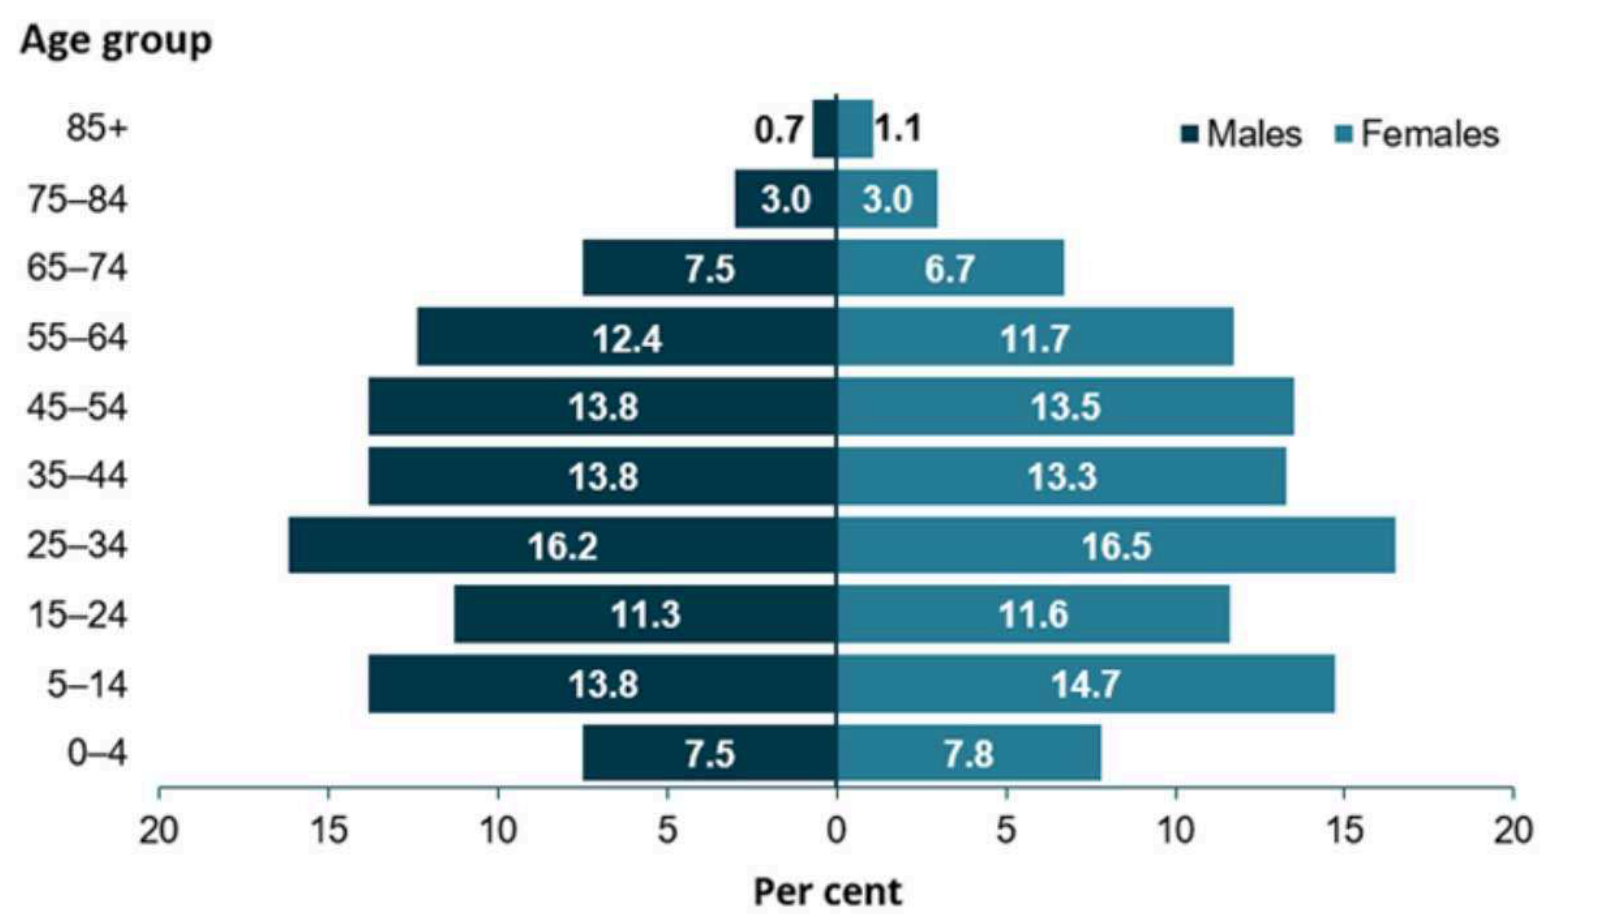
\includegraphics[width=0.95\linewidth]{img/di_age.png}\end{center}
\ptesub{范文 Model Answer（平台参考）}
\begin{modelbox}
The following graph gives information about percentages by age and sex. The items include age groups, female and male. According to this graph, in male, the value of eighty-five plus is around zero point seven, and that of seventy-five to eighty-four is higher, which is around three. You can see from this graph that the highest percentage of female is in twenty-five to thirty-four, above sixteen point five. What's more, the lowest share of male is zero point seven, for those above eighty-five. To sum up, the two areas have similar age distributions.
\end{modelbox}
\zh{该图按年龄和性别给出人口百分比，含各年龄段、女性与男性。据图，男性中 85 岁以上占比最低（约 0.7\%），75–84 岁略高（约 3\%）。女性占比最高在 25–34 岁，超过 16.5\%。男性占比最低为 85 岁以上（0.7\%）。总之，男女两侧的年龄分布相似。}
\smallskip\par{\footnotesize\color{gray}你的作答评测（AI 语音识别）：}
\begin{asrbox}
\sy{ok look at} \sg{these} \sy{pictures we can seize a x is present and} \sg{the} \sy{white is agent group and} \sg{as} \sy{below the left is may lands a right} \sy{is female} \sg{and} \sy{we can see that from twenty five to thirty four is} \sg{the} \sy{will} \sr{stir} \sy{a large people and} \sy{strewn t five} \sg{eight} \sy{choose a} \sy{thirty four for the females is the most part of them in like} \sy{eighteen five}
\end{asrbox}
{\small 评分：内容 \sfull{4.7/5}\quad·\quad 发音 \spart{71/90}\quad·\quad 流利度 \szero{33/90}}
\end{qblock}

\begin{qblock}{DI 2\quad \#567\ \ World Mobile Brands（澳洲手机品牌饼图）}{总分 \textcolor{cAccent}{\bfseries 55} / 90}
\begin{center}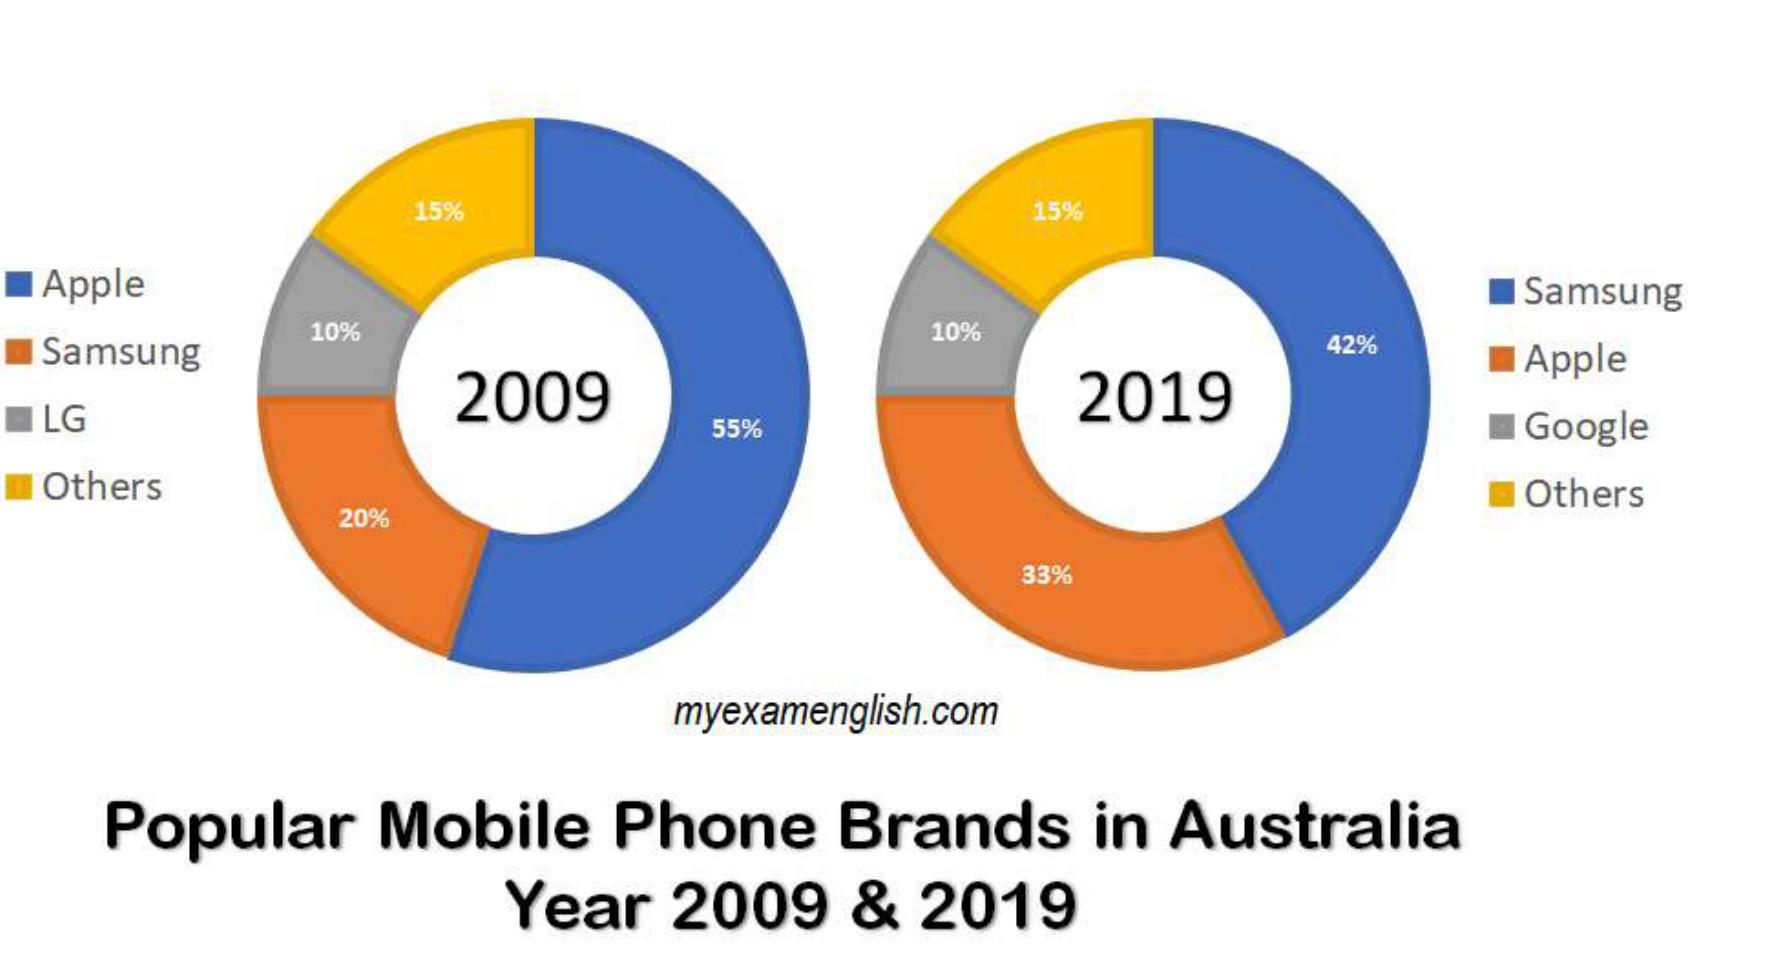
\includegraphics[width=0.86\linewidth]{img/di_phones.png}\end{center}
\ptesub{范文 Model Answer（平台参考）}
\begin{modelbox}
This pie chart gives information about popular mobile phone brands in Australia. From the chart we can see mobile phone brands include Apple, Samsung, LG and others. In two thousand and nine, Apple is the largest one, about fifty-five percent, followed by Samsung, about twenty percent. In twenty nineteen, Apple declines to thirty-three percent, and Samsung rises to forty-two percent. LG and others remain around ten percent and fifteen percent.
\end{modelbox}
\zh{该饼图给出澳大利亚流行手机品牌的信息，品牌包括 Apple、Samsung、LG 及其他。2009 年 Apple 最大（约 55\%），其次 Samsung（约 20\%）。2019 年 Apple 降到 33\%，Samsung 升到 42\%；LG 与其他大致保持在 10\% 和 15\%。}
\smallskip\par{\footnotesize\color{gray}你的作答评测（AI 语音识别）：}
\begin{asrbox}
\sg{ok look} \sy{at} \sg{this} \sg{chart is about popular mobile phone brands in} \sg{australia year in nineteen nine and} \sy{nineteen nineteen and} \sy{twenty nineteen} \sr{a} \sg{we can see that ins} \sg{a left is about} \sy{twenty} \sg{and} \sg{nine is the most popular mobile phone brand is apple and from} \sg{the left} \sr{is} \sy{a twenty nineteen} \sg{the most popular} \sy{a} \sg{mobile phone} \sg{is still} \sy{is} \sy{essential} \sg{and} \sg{the next year april}
\end{asrbox}
{\small 评分：内容 \sfull{4.5/5}\quad·\quad 发音 \spart{73/90}\quad·\quad 流利度 \szero{35/90}}
\end{qblock}

\begin{qblock}{DI 3\quad \#576\ \ European Countries（欧洲地图）}{总分 \textcolor{cAccent}{\bfseries 48} / 90}
\begin{center}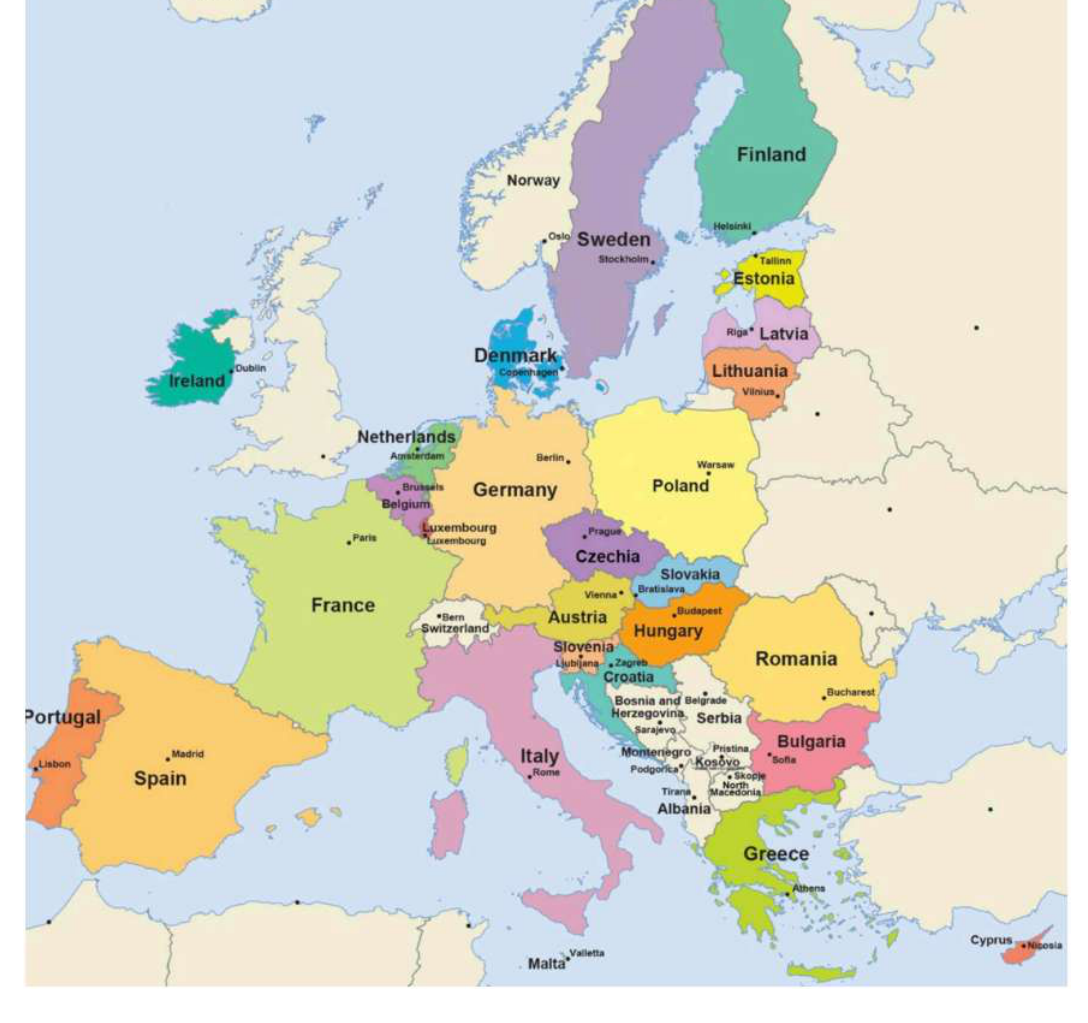
\includegraphics[width=0.52\linewidth]{img/di_map.png}\end{center}
\ptesub{范文 Model Answer（平台参考）}
\begin{modelbox}
The following graph gives information about Europe. Positions of different countries are displayed on the map. At the central area, we can see Austria, Germany, Poland and Czechia. In the left area, there lie Ireland and Portugal. According to this graph, the largest country is Russia, which is located on the right side. In comparison, small countries include Denmark and Belgium. In conclusion, there are many European countries shown on the map.
\end{modelbox}
\zh{该图给出关于欧洲的信息，地图上标出各国位置。中部可见奥地利、德国、波兰和捷克；左侧是爱尔兰和葡萄牙。据图，最大的国家是俄罗斯，位于右侧；相比之下小国包括丹麦和比利时。总之，地图展示了许多欧洲国家。}
\smallskip\par{\footnotesize\color{gray}你的作答评测（AI 语音识别）：}
\begin{asrbox}
\sg{look at} \sg{this} \sy{image} \sg{a} \sg{we can} \sg{say it's a map} \sy{of} \sy{about european} \sy{a} \sg{like} \sy{australia and romania and g choose and we can see the} \sy{span is ins} \sg{a} \sr{deft} \sy{blows a maps and we can see is a} \sg{feel} \sy{and is a} \sy{ons um} \sy{a bit slow} \sg{and} \sy{a force of the map} \sg{and} \sy{the} \sy{germany and} \sg{australia is in} \sy{the} \sg{center of the map}
\end{asrbox}
{\small 评分：内容 \sfull{4.5/5}\quad·\quad 发音 \spart{64/90}\quad·\quad 流利度 \szero{28/90}}
\end{qblock}

% ============================================================
\ptetask{RTS 情景应答}{Respond to a Situation · 恰当性 / 90　发音 / 90　流利度 / 90}

\begin{qblock}{RTS 1\quad \#20\ \ Barbecue Party}{总分 \textcolor{cAccent}{\bfseries 24} / 90}
\ptesub{情景 Situation}
\begin{promptbox}
You've organized a barbecue with your friends at your place. However, upon their arrival, you notice some of your friends are using your kitchen utensils carelessly. You need to remind everyone to handle the utensils with care to maintain their quality and keep ourselves safe. What would you say to your friends?
\end{promptbox}
\zh{你在家组织了一场烧烤聚会。朋友们到了之后，你发现有人在随意使用你的厨房用具。你需要提醒大家小心使用，以保持用具完好并确保大家的安全。你会对朋友们说什么？}
\ptesub{参考答案 Model Answer（平台参考）}
\begin{modelbox}
Hey everyone, thanks for coming over for the barbecue! Just a quick heads up, let's be careful with the kitchen utensils to avoid any accidents. I noticed some of them were getting a bit banged up. It's important to handle them with care to keep them in good shape and prevent any injuries. Let's enjoy the barbecue and make sure we clean up properly afterward. Thanks for understanding!
\end{modelbox}
\zh{大家好，谢谢来参加烧烤！提醒一下，咱们小心用厨房用具、别出意外。我注意到有些已经有点磕碰了。轻拿轻放、好好爱惜，既能保持完好也能防止受伤。咱们安全地享受烧烤，结束后一起收拾干净。谢谢理解！}
\smallskip\par{\footnotesize\color{gray}你的作答评测（AI 语音识别）：}
\begin{asrbox}
\sg{hi} \sr{i} \sg{notice that} \sr{some} \sg{of my friends are using} \sy{a} \sg{my kitchen} \sy{uses} \sy{careless i think i need to remind everyone to handles a} \sr{announces} \sg{with care} \sg{to maintain} \sy{your quality and} \sy{keep ourselves safe so i should say that you should handle your own} \sy{immunities to care about your own qualities and keep ourselves} \sy{safe}
\end{asrbox}
{\small 评分：恰当性 \spart{40/90}\quad·\quad 发音 \szero{21/90}\quad·\quad 流利度 \szero{19/90}}
\end{qblock}

\begin{qblock}{RTS 2\quad \#21\ \ Team-building Activity}{总分 \textcolor{cAccent}{\bfseries 19} / 90}
\ptesub{情景 Situation}
\begin{promptbox}
You've organized a team-building activity for your colleagues at a local park. However, upon arrival, you notice some team members are not participating actively and seem disengaged. You need to remind everyone of the importance of teamwork and encourage active participation to maximize the benefits of the activity. What would you say to your colleagues?
\end{promptbox}
\zh{你为同事们在当地公园组织了一次团建。到了之后，你发现有些成员参与不积极、显得心不在焉。你需要提醒大家团队合作的重要性，并鼓励积极参与，以最大化活动收益。你会对同事们说什么？}
\ptesub{参考答案 Model Answer（平台参考）}
\begin{modelbox}
Hey everyone, thanks for joining us for today's activity! Let's make sure we're all actively participating to get the most out of it. Remember, teamwork is key to our success, and by working together, we can achieve great things. Let's engage in the activities, share ideas, and support each other throughout. Together, we can strengthen our bond as a team and accomplish our goals more effectively. Let's dive in and make the most of this opportunity!
\end{modelbox}
\zh{大家好，谢谢参加今天的活动！咱们都积极参与，才能收获最多。记住，团队合作是成功的关键，齐心协力就能成就大事。让我们投入活动、分享想法、互相支持。一起增强团队凝聚力，更高效地达成目标。全情投入，充分利用这次机会！}
\smallskip\par{\footnotesize\color{gray}你的作答评测（AI 语音识别）：}
\begin{asrbox}
\sg{hi} \sr{i} \sg{think i have} \sy{noticed} \sg{that sound} \sr{him} \sg{members are not} \sy{participating activity and seems} \sy{disease} \sr{juice} \sg{i think} \sr{i} \sg{need to} \sg{remind everyone} \sy{of you} \sg{to} \sy{the importance of teamwork and} \sy{encourage active participant to} \sr{maximize} \sg{the benefit of} \sy{the t} \sg{so} \sy{i should i should say that every one} \sy{of our team should} \sg{know} \sr{the} \sy{importance} \sg{of} \sy{the} \sy{teamwork and you should be active um} \sg{be outgoing that's all}
\end{asrbox}
{\small 评分：恰当性 \spart{34/90}\quad·\quad 发音 \szero{14/90}\quad·\quad 流利度 \szero{15/90}\quad{\footnotesize\color{gray}（答题用时 01:30）}}
\end{qblock}

\begin{qblock}{RTS 3\quad \#22\ \ Community Garden Project}{总分 \textcolor{cAccent}{\bfseries 29} / 90}
\ptesub{情景 Situation}
\begin{promptbox}
You've organized a community garden project with your neighbors, and everyone's excited to start planting. However, upon arrival, you notice some garden beds are neglected, with weeds growing rampant. You need to remind everyone of their responsibility to maintain their assigned plots to ensure the success of the garden. What would you say to your neighbors?
\end{promptbox}
\zh{你和邻居们组织了一个社区花园项目，大家都很期待开始种植。到了之后，你发现有些菜畦无人打理、杂草疯长。你需要提醒大家有责任维护各自负责的地块，以确保花园成功。你会对邻居们说什么？}
\ptesub{参考答案 Model Answer（平台参考）}
\begin{modelbox}
Hey everyone, thanks for being part of our project. But I noticed some of the garden beds are a bit neglected, with weeds taking over. Let's all remember our responsibility to maintain our assigned plots. Weeding regularly and keeping the beds tidy will help ensure the success of our garden. Together, we can create a beautiful and thriving green space for everyone to enjoy. Let's work together to keep our garden healthy and flourishing!
\end{modelbox}
\zh{大家好，谢谢参与这个项目。不过我注意到有些菜畦有点荒了、杂草丛生。咱们都记得自己有责任维护各自的地块。定期除草、保持整洁，有助于花园成功。齐心协力，我们能打造一个美丽繁茂、人人享受的绿色空间。一起努力让花园健康茂盛！}
\smallskip\par{\footnotesize\color{gray}你的作答评测（AI 语音识别）：}
\begin{asrbox}
\sg{hi i have notice that some gardens fields} \sy{are} \sr{neglected} \sy{whiz} \sy{growing rapids i think i need to remind everyone of their} \sg{responsibility to} \sr{maintain} \sg{their} \sr{asylum} \sy{plots} \sg{to ensure the} \sg{success of the garden so i should say that} \sr{do} \sg{other things} \sy{to a} \sr{maintains era} \sy{science} \sr{abroad} \sg{to ensure the success of their} \sg{gardens}
\end{asrbox}
{\small 评分：恰当性 \spart{44/90}\quad·\quad 发音 \szero{25/90}\quad·\quad 流利度 \szero{24/90}}
\end{qblock}

% ============================================================
\ptetask{ASQ 简答}{Answer Short Question · 题目 + 参考答案 + 翻译}

{\small\color{gray} 共 6 题（取自口语题目卷）。下方为题目、参考答案与中文翻译；你的作答未截图，此处不收录。}\smallskip

\newcommand{\asqitem}[5]{%  #1=ID #2=Q(en) #3=Q(zh) #4=A(en) #5=A(zh)
  \par\smallskip{\small\textbf{\##1}\quad #2}\par
  \zh{#3}\par
  {\small\textbf{参考答案 }\textcolor{cFix}{#4}}\ {\footnotesize\color{gray}（#5）}\par}

\begin{notebox}
\asqitem{1189}{If someone tells you the truth, what is the opposite?}{如果有人对你说真话，相反（说假话）的是什么？}{Falsity / falseness / untruth}{虚假、谎言}
\asqitem{1191}{What is a person called whose job is to write news for newspapers?}{以为报纸撰写新闻为职业的人叫什么？}{Journalist}{记者}
\asqitem{1190}{What is the large, flat surface that films are shown on?}{放映电影所用的那块又大又平的表面叫什么？}{Screen}{银幕、屏幕}
\asqitem{1188}{What is another way to say the arrangement of musical notes in a tune?}{乐曲中音符的排列还可以怎么称呼？}{Melody}{旋律}
\asqitem{1187}{What is in the opposite direction from the head?}{与头部相反方向的（身体部位）是什么？}{Foot}{脚}
\asqitem{1126}{What is the scientific study of rocks?}{对岩石进行的科学研究叫什么？}{Geology}{地质学}
\end{notebox}

\clearpage
% ===== sec_reading_body.tex =====
% ===================== 阅读 Reading =====================
\ptesection{阅读}{Reading · FIB + MCM + RO + MCS}{42}

\vspace{1mm}
{\small\color{gray} 本部分依据「阅读1 / 阅读2」逐题誊录。题型：\textbf{FIB} 读写填空（下拉选词）、\textbf{FIB(R)} 读填空（拖词入空）、
\textbf{MCM} 多选、\textbf{RO} 段落重排、\textbf{MCS} 单选。每题保留：\textbf{文章（含填空/选择答案）+ 中文翻译 + 选项 + 平台中文解析（根据原文 + 解题思路）+ 评分}。}
\vspace{1mm}

\begin{notebox}
{\footnotesize 标注：填空/选择处 {\color{cFix}\ding{51}\,绿=选对}；{\color{cWrong}\ding{55}\,红删除线=选错}，其后 {\footnotesize\color{cFix}(答案: 正确词)} 给正确答案。
选项里**加粗**的是正确项。共 16 题全部收录（阅读1 = Q1–Q10，阅读2 = Q11–Q16）。}
\end{notebox}

% =================== Q1 ===================
\begin{qblock}{Q1\quad FIB \#74\ \ Good Looks in Votes}{读写填空 · 评分 \textcolor{cAccent}{\bfseries 2 / 4}}
\ptesub{文章 Passage（含填空作答）}
\begin{promptbox}
It is tempting to try to prove that good looks win votes, and many academics have tried. The \rok{difficulty} is that beauty is in the eye of the \rno{audience}{beholder}, and you cannot behold a politician's face without a veil of extraneous prejudice getting in the way. Does George Bush possess a disarming grin, or a facetious \rno{binge}{smirk}? It's hard to find anyone who can look at the president without assessing him politically as well as \rok{physically}.
\end{promptbox}
\zh{想证明“颜值能赢得选票”很有诱惑力，许多学者也尝试过。难点在于“情人眼里出西施”——你看一位政客的脸时，总有一层无关的偏见挡在中间。乔治·布什是有一种令人放松的笑容，还是一种假笑？很难找到谁能在看总统时，不在政治层面、同时也在外貌层面对他做出评判。}
\ptesub{选项 Choices}
{\small
1.\ principle,\ idea,\ \textbf{difficulty},\ concept\\
2.\ people,\ \textbf{beholder},\ builder,\ audience\\
3.\ smell,\ complexion,\ \textbf{smirk},\ binge\\
4.\ culturally,\ \textbf{physically},\ economically,\ individually}
\ptesub{解析 Explanation}
\begin{notebox}\footnotesize
\textbf{1.\ difficulty} —— 根据原文：The \_\_\_ is that beauty is in the eye of the beholder…；此处需名词表“难处”，故 difficulty；principle 原则、idea 想法、concept 概念语意不合。\textbf{思路：单句理解}。\\[2pt]
\textbf{2.\ beholder} —— 固定搭配 \emph{beauty is in the eye of the beholder}（情人眼里出西施）；people 人们、builder 建造者、audience 观众均不合。\textbf{思路：固定搭配}。\\[2pt]
\textbf{3.\ smirk} —— 根据原文：Does George Bush possess a disarming grin, or a facetious \_\_\_? 与 grin 并列、需含贬义的名词，故 smirk（假笑）；smell 气味、complexion 肤色、binge 狂欢不合。\textbf{思路：单句理解}。\\[2pt]
\textbf{4.\ physically} —— 根据原文：…assessing him politically as well as \_\_\_；与 politically 并列，按逻辑选 physically；culturally 文化上、economically 经济上、individually 个人地不合。\textbf{思路：上下文逻辑}。
\end{notebox}
\end{qblock}

% =================== Q2 ===================
\begin{qblock}{Q2\quad FIB \#50\ \ Underground Houses}{读写填空 · 评分 \textcolor{cAccent}{\bfseries 2 / 5}}
\ptesub{文章 Passage（含填空作答）}
\begin{promptbox}
Underground houses have many advantages over conventional housing. Unlike conventional homes, they can be built on \rno{overhead}{steep} surfaces and can maximize space in small areas by going below the surface. In addition, the materials excavated in construction can be used in the building process. Underground houses have less surface area so fewer building materials are used, and \rok{maintenance} costs are lower. They are also wind, fire, and earthquake resistant, providing a secure and safe environment in extreme weather. One of the greatest benefits of underground living is energy \rno{consistency}{efficiency}. The earth's subsurface temperature remains stable, so underground dwellings benefit from geothermal mass and heat exchange, staying cool in the summer and warm in the winter. This saves around 80\% in energy costs. By \rno{inventing}{incorporating} solar design this energy bill \rok{can be reduced} to zero, providing hot water and heat to the home all year round.
\end{promptbox}
\zh{地下房屋相比传统住宅有许多优势。与传统住宅不同，它们可以建在陡峭的地面上，并通过向地下发展、在狭小空间里最大化利用面积。此外，施工中挖出的材料还能用于建造过程。地下房屋表面积更小，用的建筑材料更少，维护成本也更低。它们还能抗风、抗火、抗震，在极端天气下提供安全的环境。地下居住最大的好处之一是能源效率：地表以下温度稳定，地下住宅因而受益于地热与热交换，夏凉冬暖，可节省约 80\% 的能源开支。通过引入太阳能设计，这笔能源账单可被降至零，全年为家庭提供热水和供暖。}
\ptesub{选项 Choices}
{\small
1.\ geometric,\ flat,\ overhead,\ \textbf{steep}\\
2.\ \textbf{maintenance},\ heating,\ buoyancy,\ facility\\
3.\ ratio,\ consistency,\ \textbf{efficiency},\ renewal\\
4.\ intriguing,\ initiating,\ \textbf{incorporating},\ inventing\\
5.\ has reduced,\ \textbf{can be reduced},\ can reduce,\ has been reduced}
\ptesub{解析 Explanation}
\begin{notebox}\footnotesize
\textbf{1.\ steep} —— 根据原文：they can be built on \_\_\_ surfaces…；可建在“陡峭”的地面上，故 steep；geometric 几何的、flat 平的、overhead 头顶上的 不合。\textbf{思路：单句理解}。\\[2pt]
\textbf{2.\ maintenance} —— 根据原文：…fewer building materials are used, and \_\_\_ costs are lower；面积小、维修费用低，故 maintenance（维护）。\textbf{思路：单句理解}。\\[2pt]
\textbf{3.\ efficiency} —— 结合下文 \emph{This saves around 80\% in energy costs}（省约 80\% 能耗），故能源“效率”efficiency；ratio 比率、consistency 浓度、renewal 更新 不合。\textbf{思路：上下文理解}。\\[2pt]
\textbf{4.\ incorporating} —— 根据原文：By \_\_\_ solar design… providing hot water…；需“引入/纳入”太阳能设计，故 incorporating；intriguing 引发、initiating 发起、inventing 发明 不合。\textbf{思路：动宾搭配}。\\[2pt]
\textbf{5.\ can be reduced} —— 主语 energy bill 与“减少”是被动关系，且为假设、非已完成，故被动 can be reduced；has reduced、can reduce、has been reduced 不合。\textbf{思路：时态 + 被动语态}。
\end{notebox}
\end{qblock}

% =================== Q3 ===================
\begin{qblock}{Q3\quad FIB \#3\ \ Intelligence Comparison}{读写填空 · 评分 \textcolor{cAccent}{\bfseries 2 / 5}}
\ptesub{文章 Passage（含填空作答）}
\begin{promptbox}
Comparing the intelligence of animals of different species is difficult: how do you compare a dolphin and a horse? Psychologists have a technique for looking at intelligence that \rok{does} not require the cooperation of the animal involved. The relative size of an individual's brain is a reasonable indication of intelligence. Comparing \rno{with}{across} species is not as simple as generally expected. An elephant will have a larger brain than a human has simply because it is a large beast. \rno{Otherwise}{Instead}, we use the Cephalization index, which compares the size of an animal's brain with the size of its body. Based on the Cephalization index, the brightest animals on the planet are humans, \rok{followed} by great apes, porpoises and elephants. As a general \rno{principle}{rule}, animals that hunt for a living (like canines) are smarter than strict vegetarians (you don't need much intelligence to outsmart a leaf of lettuce). Animals that live in social groups are always smarter and have larger EQ's than solitary animals.
\end{promptbox}
\zh{比较不同物种动物的智力很难：你怎么比较一只海豚和一匹马？心理学家有一套观察智力的方法，它无需相关动物的配合——个体大脑的相对大小就是智力的一个合理指标。跨物种比较并不像一般以为的那么简单：大象的脑比人大，只是因为它体型大。于是我们改用“脑化指数”，把动物大脑的大小与其身体大小相比较。按脑化指数，地球上最聪明的动物是人类，其次是类人猿、海豚和大象。一般来说，以狩猎为生的动物（如犬科）比纯素食动物更聪明（要智胜一片生菜并不需要多少智力）。群居动物总是比独居动物更聪明、EQ 更高。}
\ptesub{选项 Choices}
{\small
1.\ can,\ do,\ did,\ \textbf{does}\\
2.\ \textbf{across},\ to,\ through,\ with\\
3.\ Then,\ \textbf{Instead},\ Because,\ Otherwise\\
4.\ \textbf{followed},\ follows,\ follow,\ following\\
5.\ theory,\ principal,\ \textbf{rule},\ principle}
\ptesub{解析 Explanation}
\begin{notebox}\footnotesize
\textbf{1.\ does} —— 根据原文：…a technique…that \_\_\_ not require the cooperation of the animal involved；需助动词、第三人称单数现在时，故 does；can/did/do 不匹配。\textbf{思路：主谓一致 + 时态}。\\[2pt]
\textbf{2.\ across} —— 根据原文：Comparing \_\_\_ species…；表“跨/不同物种间”比较，故 across；to/through/with 不合。\textbf{思路：单句理解}。\\[2pt]
\textbf{3.\ Instead} —— 根据原文：\_\_\_, we use the Cephalization index…；与前句形成转折，故副词 Instead；Then/Because/Otherwise 不合。\textbf{思路：单句理解（转折）}。\\[2pt]
\textbf{4.\ followed} —— 根据原文：…humans, \_\_\_ by great apes…；表“其次/紧随其后”，过去分词作后置定语，故 followed；follows/follow/following 不合。\textbf{思路：过去分词}。\\[2pt]
\textbf{5.\ rule} —— 固定搭配 \emph{as a general rule}（一般来说）；theory 理论、principal 校长、principle 法则 不合。\textbf{思路：固定搭配}。
\end{notebox}
\end{qblock}

% =================== Q4 ===================
\begin{qblock}{Q4\quad FIB \#70\ \ Mini Helicopter}{读写填空 · 评分 \textcolor{cAccent}{\bfseries 2 / 5}}
\ptesub{文章 Passage（含填空作答）}
\begin{promptbox}
A mini helicopter modelled on flying tree seeds could soon be flying overhead. Evan Ulrich and colleagues at the University of Maryland in College Park \rno{turned in}{turned to} the biological world for inspiration to build a scaled-down helicopter that could mimic the properties of full-size aircraft. The complex \rok{design} of full-size helicopters gets less efficient when shrunk, meaning that standard mini helicopters expend most of their power simply fighting to stay stable in the air. The researchers realized that a simpler aircraft designed to stay stable passively would use much less power and reduce manufacturing costs to boot. It turns out that nature \rno{is beating}{had beaten} them to it. The seeds of trees have a single-blade structure that \rok{allows} them to fly far away and drift safely to the ground. These seeds need no engine to \rno{fly}{spin} through the air, thanks to a process called autorotation. By analyzing the behavior of the samara with high-speed cameras, Ulrich and his team were able to copy its design.
\end{promptbox}
\zh{一种以飞行树种子为原型的微型直升机可能很快就会在头顶飞行。马里兰大学帕克分校的 Evan Ulrich 及同事转向生物界寻找灵感，想造一架能模仿全尺寸飞行器特性的缩小版直升机。全尺寸直升机复杂的设计在缩小后效率会下降，这意味着普通微型直升机的大部分动力都耗在勉力维持空中稳定上。研究者意识到，一架靠被动方式保持稳定的更简单飞行器会省电得多，还能降低制造成本。事实证明，大自然早已抢先一步：树的种子有一种单叶片结构，能让它们飞得很远并安全飘落到地面。借助一种叫“自转”的过程，这些种子无需发动机就能在空中旋转。通过用高速摄像机分析翅果（samara）的运动，Ulrich 团队得以复制其设计。}
\ptesub{选项 Choices}
{\small
1.\ \textbf{turned to},\ turned for,\ turned in,\ turned off\\
2.\ overhaul,\ gauge,\ imagination,\ \textbf{design}\\
3.\ is beating,\ was beaten,\ \textbf{had beaten},\ beaten\\
4.\ had allowed,\ allowed,\ \textbf{allows},\ will allow\\
5.\ \textbf{spin},\ fluctuate,\ drift,\ fly}
\ptesub{解析 Explanation}
\begin{notebox}\footnotesize
\textbf{1.\ turned to} —— 根据原文：…colleagues \_\_\_ the biological world for inspiration…；转向自然界寻求灵感，故 turned to（求助于）；turned in/for/off 不合。\textbf{思路：单句理解}。\\[2pt]
\textbf{2.\ design} —— 根据原文：The \_\_\_ of full-size helicopters gets less efficient when shrunk…；指“设计”，故 design；overhaul 检修、gauge 仪表、imagination 想象 不合。\textbf{思路：上下文理解}。\\[2pt]
\textbf{3.\ had beaten} —— 根据原文：It turns out that nature \_\_\_ them to it；\emph{beat sb. to it}（抢先一步），与 realized 等过去时呼应，表“过去的过去”，故过去完成 had beaten；is beating/was beaten/beaten 不合。\textbf{思路：时态}。\\[2pt]
\textbf{4.\ allows} —— 根据原文：…a single-blade structure that \_\_\_ them to fly far away…；定语从句谓语、一般现在时，故 allows；had allowed/allowed/will allow 时态不合。\textbf{思路：时态}。\\[2pt]
\textbf{5.\ spin} —— 根据原文：These seeds need no engine to \_\_\_ through the air, thanks to a process called autorotation；autorotation（自旋），故 spin（旋转）；fluctuate 波动、drift 漂流、fly 飞 不合。\textbf{思路：单句理解}。
\end{notebox}
\end{qblock}

% =================== Q5 ===================
\begin{qblock}{Q5\quad FIB \#290\ \ Power Mix}{读写填空 · 评分 \textcolor{cAccent}{\bfseries 3 / 5}}
\ptesub{文章 Passage（含填空作答）}
\begin{promptbox}
Imagine a time in the not too distant future when your power comes from a seamless mix of renewable energy and traditional sources. It is delivered by a grid that manages thousands of windmills and hundreds of thousands of customers. Computer \rno{controlling}{controlled}, the grid is able to manage instant variations in supply and demand and provides a real time power balance. Far more complex than anything \rok{in} existence today, it is the smart grid. This technology is a new frontier in power supply and seen as a green solution to current outdated management systems. When introduced, smart grids will result in energy savings and will allow consumers a choice in their electricity charges and to be able to select the cheapest time \rno{pins}{slots}. The difficulty for the energy industry is that smart grids \rok{do not exist} in reality and the power companies cannot experiment with existing supplies. Without an actual grid to conduct research on, Professor Wu has had to design a simulated laboratory including input from theoretical wind generators and solar panels to feed into a constantly operating system. For an authentic approach researchers built various types of equipment failures \rok{into} the grid to test the system. And it works.
\end{promptbox}
\zh{设想在不远的将来，你的电力来自可再生能源与传统能源的无缝组合，由一张管理着成千上万台风车、数十万用户的电网输送。在计算机控制下，电网能管理供需的瞬时变化，提供实时的电力平衡。它远比当今现存的任何系统都复杂——这就是智能电网。这项技术是电力供应的新前沿，被视为解决当前陈旧管理系统的绿色方案。智能电网一旦引入，将带来节能，并让消费者在电费上有选择权、能挑选最便宜的时段。能源行业的难处在于：智能电网在现实中并不存在，电力公司无法用现有供电做实验。由于没有真实电网可供研究，Wu 教授只得设计一个模拟实验室，引入理论风力发电机和太阳能板的输入，接入一个持续运行的系统。为贴近真实，研究者在电网中植入各种类型的设备故障来测试系统。结果——它奏效了。}
\ptesub{选项 Choices}
{\small
1.\ \textbf{controlled},\ has controlled,\ controls,\ controlling\\
2.\ with,\ without,\ of,\ \textbf{in}\\
3.\ cuts,\ pins,\ points,\ \textbf{slots}\\
4.\ does not exist,\ \textbf{do not exist},\ are not existing,\ not exist\\
5.\ \textbf{into},\ of,\ onto,\ above}
\ptesub{解析 Explanation}
\begin{notebox}\footnotesize
\textbf{1.\ controlled} —— 根据原文：Computer \_\_\_, the grid is able to…（独立主格结构）；Computer 与 control 为被动关系，用过去分词 controlled。\textbf{思路：独立主格 / 非谓语}。\\[2pt]
\textbf{2.\ in} —— 固定搭配 \emph{in existence}（现存的）：anything \_\_\_ existence today，故 in。\textbf{思路：介词 / 固定搭配}。\\[2pt]
\textbf{3.\ slots} —— 根据原文：…select the cheapest time \_\_\_；\emph{time slots}（时段），故 slots；cuts/pins/points 不合。\textbf{思路：词组搭配}。\\[2pt]
\textbf{4.\ do not exist} —— 根据原文：…smart grids \_\_\_ in reality…；主语复数、一般现在时否定，故 do not exist；does not exist/are not existing/not exist 不合。\textbf{思路：主谓一致}。\\[2pt]
\textbf{5.\ into} —— 根据原文：…built various types of equipment failures \_\_\_ the grid…；表“放入…其中”，故 into（与上文 feed into 呼应）；of/onto/above 不合。\textbf{思路：介词}。
\end{notebox}
\end{qblock}

% =================== Q6 ===================
\begin{qblock}{Q6\quad MCM-R \#52\ \ History of Sleep}{多选 Multiple Answers · 评分 \textcolor{cAccent}{\bfseries 0 / 3}}
\ptesub{文章 Passage}
\begin{promptbox}
September 2, 1752, was a great day in the history of sleep. That Wednesday evening, millions of British subjects in England and the colonies went peacefully to sleep and did not wake up until twelve days later. Behind this feat of narcoleptic prowess was not some revolutionary hypnotic technique or miraculous pharmaceutical discovered in the West Indies. It was, rather, the British Calendar Act of 1751, which declared the day after Wednesday 2nd to be Thursday 14th. Prior to that cataclysmic September evening, the official British calendar differed from that of continental Europe by eleven days---that is, September 2 in London was September 13 in Paris, Lisbon, and Berlin. The discrepancy had sprung from Britain's continued use of the Julian calendar, which had been the official calendar of Europe from its invention by Julius Caesar (after whom it was named) in 45 B.C. until the decree of Pope Gregory XIII in 1582. Caesar's calendar, which consisted of eleven months of 30 or 31 days and a 28-day February (extended to 29 days every fourth year), was actually quite accurate: it erred from the real solar calendar by only 11.5 minutes a year. After centuries, though, even a small inaccuracy like this adds up. By the sixteenth century, it had put the Julian calendar behind the solar one by 10 days. In Europe, in 1582, Pope Gregory XIII ordered the advancement of the Julian calendar by 10 days and introduced a new corrective device to curb further error: century years such as 1700 or 1800 would no longer be counted as leap years, unless they were (like 1600 or 2000) divisible by 400.
\end{promptbox}
\zh{1752 年 9 月 2 日是睡眠史上“伟大”的一天。那个周三晚上，英格兰及其殖民地的数百万英国臣民安然入睡，直到十二天后才醒来。这桩“嗜睡壮举”的背后，并非什么革命性的催眠术或在西印度群岛发现的神奇药物，而是 1751 年的《英国历法法案》——它宣布周三 2 日的次日即为周四 14 日。在那个翻天覆地的九月夜晚之前，英国官方历法与欧洲大陆相差十一天——伦敦的 9 月 2 日，就是巴黎、里斯本和柏林的 9 月 13 日。这一差异源于英国一直沿用儒略历：自公元前 45 年尤利乌斯·凯撒发明（历法因他得名）起，到 1582 年教皇格里高利十三世颁布敕令为止，它都是欧洲的官方历法。凯撒的历法由 11 个 30 或 31 天的月份和一个 28 天的二月（每四年延长为 29 天）组成，其实相当准确：每年与真实太阳历仅差 11.5 分钟。但几个世纪累积，即便这点小误差也会叠加；到 16 世纪，儒略历已比太阳历落后 10 天。1582 年，教皇下令把儒略历提前 10 天，并引入新纠错机制：1700、1800 这样的世纪年不再算闰年，除非（像 1600、2000）能被 400 整除。}
\ptesub{题目 Question}
\begin{notebox}\small What factors were involved in the disparity between the calendars of Britain and Europe in the 17th century?\end{notebox}
\ptesub{选项 Choices（多选）}
{\small
A）the provisions of the British Calendar Act of 1751\\
{\color{cFix}\textbf{B）Britain's continued use of the Julian calendar}}\\
{\color{cFix}\textbf{C）the accrual of very minor differences between the calendar used in Britain and real solar events}}\\
D）the failure to include years divisible by four as leap years\\
{\color{cFix}\textbf{E）the decree of Pope Gregory XIII}}\\
F）revolutionary ideas which had emerged from the West Indies\\
G）Britain's use of a calendar consisting of twelve months rather than eleven}
\smallskip\par
{\small 正确答案 \textcolor{cFix}{\bfseries B, C, E}\qquad 你的答案 {\color{cWrong}\bfseries C, F}\;{\footnotesize\color{gray}（C 对、F 错；多选错选不得分）}}
\end{qblock}

% =================== Q7 ===================
\begin{qblock}{Q7\quad MCM-R \#53\ \ X-ray}{多选 Multiple Answers · 评分 \textcolor{cAccent}{\bfseries 1 / 2}}
\ptesub{文章 Passage}
\begin{promptbox}
X-ray crystallography is the study of crystal structures through X-ray diffraction techniques. When an X-ray beam bombards a crystalline lattice in a given orientation, the beam is scattered in a definite manner characterized by the atomic structure of the lattice. This phenomenon, known as X-ray diffraction, occurs when the wavelength of X-rays and the interatomic distances in the lattice have the same order of magnitude. In 1912, the German scientist Max von Laue predicted that crystals exhibit diffraction qualities. Concurrently, W. Friedrich and P. Knipping created the first photographic diffraction patterns. A year later, Lawrence Bragg successfully analyzed the crystalline structures of potassium chloride and sodium chloride using X-ray crystallography, and developed a rudimentary treatment for X-ray/crystal interaction (Bragg's Law). Bragg's research provided a method to determine a number of simple crystal structures for the next 50 years. In the 1960s, the capabilities of X-ray crystallography were greatly improved by the incorporation of computer technology. Modern X-ray crystallography provides the most powerful and accurate method for determining single-crystal structures. Structures containing 100--200 atoms now can be analyzed on the order of 1--2 days, whereas before the 1960s a 20-atom structure required 1--2 years for analysis. Through X-ray crystallography the chemical structure of thousands of organic, inorganic, organometallic, and biological compounds are determined every year.
\end{promptbox}
\zh{X 射线晶体学是通过 X 射线衍射技术研究晶体结构的学科。当 X 射线束以特定取向轰击晶格时，射线会以由晶格原子结构决定的特定方式被散射；这种现象称为 X 射线衍射，当 X 射线波长与晶格中原子间距处于同一数量级时即发生。1912 年，德国科学家马克斯·冯·劳厄预言晶体会表现出衍射特性；同期 W. 弗里德里希与 P. 克尼平制作出首批衍射照片图样。一年后，劳伦斯·布拉格用 X 射线晶体学成功分析了氯化钾、氯化钠的晶体结构，并提出 X 射线/晶体相互作用的基本处理方法（布拉格定律）。布拉格的研究为之后 50 年测定若干简单晶体结构提供了方法。20 世纪 60 年代，计算机技术的引入大大提升了其能力。现代 X 射线晶体学提供了测定单晶结构最强大、最精确的方法：含 100–200 个原子的结构如今 1–2 天即可分析，而 60 年代前一个 20 原子的结构需 1–2 年。借助 X 射线晶体学，每年都能测定数以千计的有机、无机、有机金属和生物化合物的化学结构。}
\ptesub{题目 Question}
\begin{notebox}\small Which of the following factors are consistent with the theory of X-ray crystallography?\end{notebox}
\ptesub{选项 Choices（多选）}
{\small
A）X-ray crystallization causes a reduction in the interatomic distances of wavelengths.\\
{\color{cFix}\textbf{B）X-rays are scattered according to the atomic structure of the crystal lattice.}}\\
C）The analysis of chemical compounds was only possible after the development of computer technology.\\
{\color{cFix}\textbf{D）The process can be used to determine the chemical structure of biological compounds.}}\\
E）X-rays will not diffract in crystalline substances.}
\smallskip\par
{\small 正确答案 \textcolor{cFix}{\bfseries B, D}\qquad 你的答案 {\color{cWrong}\bfseries D}\;{\footnotesize\color{gray}（漏选 B）}}
\end{qblock}

% =================== Q8 ===================
\begin{qblock}{Q8\quad RO \#307\ \ Noise and Study}{段落重排 Re-order · 评分 \textcolor{cAccent}{\bfseries 1 / 3}}
\ptesub{段落 Paragraphs（按原乱序编号）}
\begin{promptbox}\small
\textbf{1)} However, one general rule for all students is that the television seems to be more of a distraction than music or other background noise, so leave the TV off when you are reading or studying. Also, don't let yourself distracted by computer games, email, or internet surfing.\\[2pt]
\textbf{2)} Some students say that they need complete quiet to read and study.\\[2pt]
\textbf{3)} The point is, you should know the level of noise that is optimal for your own studying.\\[2pt]
\textbf{4)} Others study best in crowded, noisy rooms because the noise actually helps them concentrate.
\end{promptbox}
\zh{1）不过，对所有学生都适用的一条通则是：电视似乎比音乐或其他背景噪音更让人分心，所以读书学习时把电视关掉，也别被电脑游戏、邮件或上网分心。2）有些学生说，他们读书学习需要绝对安静。3）关键在于，你要知道最适合自己学习的噪音水平。4）另一些人在拥挤吵闹的房间里学得最好，因为噪音反而帮他们集中注意力。}
\smallskip\par
{\small 正确顺序 \textcolor{cFix}{\bfseries 2 → 4 → 3 → 1}\qquad 你的顺序 {\color{cWrong}\bfseries 2 → 1 → 4 → 3}}
\end{qblock}

% =================== Q9 ===================
\begin{qblock}{Q9\quad RO \#300\ \ GPS Tracking（GPS 定位）}{段落重排 Re-order · 评分 \textcolor{cAccent}{\bfseries 3 / 3}}
\ptesub{段落 Paragraphs（按原乱序编号）}
\begin{promptbox}\small
\textbf{1)} The collars transmitted each animal's position every four hours, for up to two years.\\[2pt]
\textbf{2)} But in 2010 and 2011, Vanessa Hull of Michigan State University and her colleagues were given permission to attach GPS tracking collars to five pandas in the Wolong National Nature Reserve in China.\\[2pt]
\textbf{3)} We know very little about wild pandas because they are so rare and live in almost impenetrable forest.\\[2pt]
\textbf{4)} The team found that the home ranges of individual pandas overlapped and on a few occasions, two animals spent several weeks in close proximity.
\end{promptbox}
\zh{1）项圈每隔四小时传送一次每只动物的位置，持续长达两年。2）但在 2010 和 2011 年，密歇根州立大学的 Vanessa Hull 及同事获准给卧龙国家级自然保护区的五只大熊猫戴上 GPS 追踪项圈。3）我们对野生大熊猫知之甚少，因为它们非常稀少、且生活在几乎无法穿越的森林里。4）团队发现，各只熊猫的活动范围相互重叠，偶尔有两只熊猫连续数周近距离共处。}
\smallskip\par
{\small 正确顺序 \textcolor{cFix}{\bfseries 3 → 2 → 1 → 4}\qquad 你的顺序 \textcolor{cFix}{\bfseries 3 → 2 → 1 → 4}\;{\footnotesize\color{gray}（全对）}}
\par{\footnotesize\color{gray}思路：先“我们知之甚少（3）”，再“2010–11 装 GPS 项圈（2）”，接着“项圈传送位置（1）”，最后“发现活动范围重叠（4）”。}
\end{qblock}

% =================== Q10 ===================
\begin{qblock}{Q10\quad FIB(R) \#483\ \ Martens' Diet}{读填空（拖词）· 评分 \textcolor{cAccent}{\bfseries 2 / 4}}
\ptesub{文章 Passage（含填空作答）}
\begin{promptbox}
Studies of pine martens in Scotland have shown that the diet varies \rok{seasonally} with small mammals, berries (in late summer/autumn) and small birds being the main foods. Recent work on a plantation has shown that martens \rok{establish} their home ranges in areas dominated by forests and \rno{lately}{dense} shrubs. Within home ranges, martens utilize areas of grassy vegetation within the forest which are typically associated with Microtus voles, for which a strong selective \rno{decision}{preference} over other small mammals is shown.
\end{promptbox}
\zh{在苏格兰对松貂的研究表明，其食物随季节变化，以小型哺乳动物、浆果（夏末/秋季）和小鸟为主要食物。一处人工林的最新研究显示，松貂把活动范围建立在以森林和茂密灌木为主的区域。在活动范围内，松貂会利用森林中通常与田鼠（Microtus voles）相关的草地植被区域——相对其他小型哺乳动物，它们对田鼠表现出强烈偏好。}
\ptesub{选项 Choices（拖词词库，多于空格数）}
{\small \textbf{seasonally}\quad \textbf{establish}\quad \textbf{dense}\quad \textbf{preference}\quad ｜\quad lately,\ decision,\ complicated（多余干扰词）}
\ptesub{解析 Explanation}
\begin{notebox}\footnotesize
\textbf{1.\ seasonally} —— 根据原文：the diet varies \_\_\_ with small mammals…；副词修饰 varies，故 seasonally（季节性地）。\textbf{思路：词性 + 单句理解}。\\[2pt]
\textbf{2.\ establish} —— 根据原文：martens \_\_\_ their home ranges…；需动词谓语“建立”，故 establish。\textbf{思路：动词谓语}。\\[2pt]
\textbf{3.\ dense} —— 根据原文：forests and \_\_\_ shrubs；需形容词修饰 shrubs，故 dense（茂密的）；lately（副词）不合。\textbf{思路：词性 + 搭配}。\\[2pt]
\textbf{4.\ preference} —— 根据原文：a strong selective \_\_\_ over other small mammals…；固定搭配 \emph{a preference for A over B}（相比 B 更偏好 A），故 preference；decision 不合。\textbf{思路：固定搭配}。
\end{notebox}
\end{qblock}

% =================== Q11 ===================
\begin{qblock}{Q11\quad FIB(R) \#165\ \ Bees' Die-off}{读填空（拖词）· 评分 \textcolor{cAccent}{\bfseries 4 / 5}}
\ptesub{文章 Passage（含填空作答）}
\begin{promptbox}
It sounds like something out of a science fiction movie --- or nightmare: millions of honeybees \rok{suddenly} dying off, their bodies never found. Scientists have \rok{named} the phenomenon `Colony Collapse Disorder', but they aren't \rno{deliberating}{united} on the reason. Theories abound as to the \rok{cause} of the mass die-off, ranging from the unlikely (cellphones affecting bees' navigational abilities) to the more \rok{plausible} though still debated (widespread pesticide use).
\end{promptbox}
\zh{这听起来像科幻电影——或噩梦：数百万只蜜蜂突然死去，却找不到它们的尸体。科学家把这一现象命名为“蜂群崩溃失调症”，但对其原因尚未达成一致。关于这场大规模死亡的原因众说纷纭，从不太可能的（手机影响蜜蜂导航能力）到更可信、但仍有争议的（农药的广泛使用）。}
\ptesub{选项 Choices（拖词词库，多于空格数）}
{\small \textbf{suddenly}\quad \textbf{named}\quad \textbf{united}\quad \textbf{cause}\quad \textbf{plausible}\quad ｜\quad deliberating,\ possibility,\ authored（多余干扰词）}
\ptesub{解析 Explanation}
\begin{notebox}\footnotesize
\textbf{1.\ suddenly} —— …millions of honeybees \_\_\_ dying off…；副词修饰 dying，故 suddenly（突然）。\textbf{思路：词性}。\\[2pt]
\textbf{2.\ named} —— Scientists have \_\_\_ the phenomenon…；\emph{name sth}（命名），现在完成 have named。\textbf{思路：动词 + 时态}。\\[2pt]
\textbf{3.\ united} —— they aren't \_\_\_ on the reason；\emph{be united on}（在…上达成一致），故 united；deliberating（审议）不合。\textbf{思路：搭配}。\\[2pt]
\textbf{4.\ cause} —— as to the \_\_\_ of the mass die-off…；名词“原因”，故 cause。\textbf{思路：词性 + 单句理解}。\\[2pt]
\textbf{5.\ plausible} —— to the more \_\_\_ though still debated…；形容词“可信的”，故 plausible。\textbf{思路：词性 + 上下文}。
\end{notebox}
\end{qblock}

% =================== Q12 ===================
\begin{qblock}{Q12\quad FIB(R) \#481\ \ Contagious Emotions}{读填空（拖词）· 评分 \textcolor{cAccent}{\bfseries 3 / 3}}
\ptesub{文章 Passage（含填空作答）}
\begin{promptbox}
As research has shown, emotions are contagious. And empaths are especially \rok{sensitive} to others' emotional energies. Because they can get easily exhausted in crowds, be drawn into codependent \rok{relationships}, exhaust themselves trying to solve others' problems, or burn out from too much caregiving. Yet empathy is also a gift that brings greater \rok{insight} and understanding. Some of the finest therapists, doctors, nurses, professors, writers, designers, musicians, artists and leaders in many have been empaths.
\end{promptbox}
\zh{研究表明，情绪会传染。共情者（empaths）对他人的情感能量尤其敏感。他们在人群中容易精疲力竭，会陷入相互依赖的关系，会因试图解决别人的问题而耗尽自己，或因过度照顾他人而倦怠。然而，共情也是一种天赋，能带来更深的洞察与理解。许多最优秀的治疗师、医生、护士、教授、作家、设计师、音乐家、艺术家与领袖，都曾是共情者。}
\ptesub{选项 Choices（拖词词库，多于空格数）}
{\small \textbf{sensitive}\quad \textbf{relationships}\quad \textbf{insight}\quad ｜\quad confusion,\ issues,\ resistant（多余干扰词）}
\ptesub{解析 Explanation}
\begin{notebox}\footnotesize
\textbf{1.\ sensitive} —— …empaths are especially \_\_\_ to others' emotional energies；be 后接形容词，故 sensitive（敏感的）；resistant 不合。\textbf{思路：词性}。\\[2pt]
\textbf{2.\ relationships} —— …be drawn into codependent \_\_\_；形容词后需名词，故 relationships（关系）；issues 不合。\textbf{思路：词性}。\\[2pt]
\textbf{3.\ insight} —— …brings greater \_\_\_；greater 后需名词，故 insight（洞察）；confusion 不合。\textbf{思路：词性 + 上下文}。
\end{notebox}
\end{qblock}

% =================== Q13 ===================
\begin{qblock}{Q13\quad FIB(R) \#465\ \ Utopias}{读填空（拖词）· 评分 \textcolor{cAccent}{\bfseries 2 / 6}}
\ptesub{文章 Passage（含填空作答）}
\begin{promptbox}
Many Utopias have been dreamed up through the ages. From Plato's Republic to Thomas More's Utopia and beyond, serious thinkers have \rno{exchanged}{envisioned} societies where people live in peace and harmony. Most of these imaginary worlds have things in common: everybody is equal and plays a part in the running of the society; nobody goes without the essentials of life; people live mostly off the land; often there is no money, and so on. Another thing they have in \rok{common} is that, to the average person, they appear distasteful or unworkable since they do not take into account ordinary human nature or feelings. Architects have got in on the act, too. After the Great Fire of London, Christopher Wren drew up plans for a reconstruction of the whole city, including \rno{horizontal}{precise} grand avenues; in the 20th century there was Le Corbusier's Radiant City in which, if you weren't in a car or didn't have one, life would have been a nightmare. Also in the 20th century, another famous architect, Frank Lloyd Wright, \rok{dreamed} up a perfect city that got no further than the drawing-board. Wright believed that what was wrong with modern cities was, in his words, rent: ideas, land, even money itself, had to be paid for. He saw this as a form of slavery and believed that modern city dwellers had no sense of themselves as productive individuals. Thus, Wright's city was to be made up of numerous individual homesteads, and the houses themselves were to be simple, functional and in \rno{pieced}{harmony} with the environment. Everyone would own enough land to grow food for himself and his family. No outsiders would be allowed to come between the citizen and what he produced, or to exploit both for money. Goods and services would all be \rno{envisioned}{exchanged}, not bought and sold for profit.
\end{promptbox}
\zh{古往今来人们构想过许多乌托邦。从柏拉图《理想国》到托马斯·莫尔《乌托邦》乃至之后，严肃的思想家们设想过种种人们和平和谐共处的社会。这些想象世界大多有共同点：人人平等、都参与社会运作；无人缺乏生活必需品；人们多半靠土地为生；往往没有货币，等等。它们还有一个共同点：在普通人看来令人反感或行不通，因为没有考虑普通人的本性与情感。建筑师们也参与其中。伦敦大火后，克里斯托弗·雷恩制定了重建全城的规划，包括精确规整的大道；20 世纪有勒·柯布西耶的“光辉城市”，在那里若你没有汽车，生活会是噩梦。同样在 20 世纪，另一位著名建筑师弗兰克·劳埃德·赖特构想了一座完美城市，却止步于图纸。赖特认为现代城市的问题在于——用他的话说——租金：理念、土地乃至金钱本身都要花钱买。他视之为一种奴役，认为现代城市居民没把自己当作有生产力的个体。因此，赖特的城市将由许多个人家园组成，房屋本身简单、实用、与环境和谐。人人拥有足够土地为自己和家人种粮；不允许外人介入公民与其产出之间、或为牟利剥削两者。商品和服务都将被交换，而非为利润买卖。}
\ptesub{选项 Choices（拖词词库，多于空格数）}
{\small \textbf{envisioned}\quad \textbf{common}\quad \textbf{precise}\quad \textbf{dreamed}\quad \textbf{harmony}\quad \textbf{exchanged}\quad ｜\quad regulated,\ paved,\ incorporated（多余干扰词）}
\ptesub{解析 Explanation}
\begin{notebox}\footnotesize
\textbf{1.\ envisioned} —— serious thinkers have \_\_\_ societies…；动词谓语“构想/设想”，故 envisioned；exchanged（交换）不合。\textbf{思路：动词 + 上下文}。\\[2pt]
\textbf{2.\ common} —— Another thing they have in \_\_\_…；\emph{have in common}（有共同点），故 common。\textbf{思路：固定搭配}。\\[2pt]
\textbf{3.\ precise} —— including \_\_\_ grand avenues；形容词“精确规整的”，故 precise；horizontal（水平的）不合。\textbf{思路：词性 + 语义}。\\[2pt]
\textbf{4.\ dreamed} —— Wright \_\_\_ up a perfect city；\emph{dream up}（凭空设想），故 dreamed。\textbf{思路：动词短语}。\\[2pt]
\textbf{5.\ harmony} —— in \_\_\_ with the environment；\emph{in harmony with}（与…和谐），故 harmony；pieced 不合。\textbf{思路：固定搭配}。\\[2pt]
\textbf{6.\ exchanged} —— Goods and services would all be \_\_\_…；被动语态、“交换”，故 exchanged；envisioned 不合。\textbf{思路：被动语态 + 上下文}。
\end{notebox}
\end{qblock}

% =================== Q14 ===================
\begin{qblock}{Q14\quad FIB(R) \#449\ \ Supply and Demand}{读填空（拖词）· 评分 \textcolor{cAccent}{\bfseries 3 / 4}}
\ptesub{文章 Passage（含填空作答）}
\begin{promptbox}
The supply of a thing, in the phrase `supply and demand', is the amount that will be offered for sale at each of a series of prices; the demand is the amount that will be bought at each of a series of prices. The principle that value depends on supply and demand means that in the case of nearly every commodity, more will be bought if the price is lowered; less will be bought if the price is \rok{raised}. Therefore sellers, if they wish to induce buyers to take more of a commodity than they are already doing, must reduce its price; if they raise its price, they will sell less. If there is a general falling-off in demand --- due, say, to trade depression --- sellers will either have to \rok{reduce} prices or put less on the \rok{market}; they will not be able to sell the same \rno{gear}{amount} at the same price. Similarly with supply. At a certain price a certain amount will be offered for sale; at a higher price more will be offered; at a lower price less. If consumers want more, they must offer a higher price; if they want less, they will probably be able to force prices down. That is the first result of a change in demand or supply.
\end{promptbox}
\zh{在“供给与需求”这一短语中，某物的供给是指在一系列价格下愿意出售的数量；需求是指在一系列价格下会被买进的数量。“价值取决于供求”这一原理意味着：对几乎每种商品而言，价格降低则买得更多，价格提高则买得更少。因此，卖方若想让买家比现在买得更多，就必须降价；若提价，就会卖得更少。若需求普遍下滑——比如因贸易萧条——卖方要么降价，要么减少投放市场的量；他们将无法以同样的价格卖出同样的数量。供给方面也类似：某一价格下会有一定数量供售，价格越高供应越多，越低越少。消费者想要更多就得出更高的价；想要更少则多半能把价格压下来。这就是供求变化的首要结果。}
\ptesub{选项 Choices（拖词词库，多于空格数）}
{\small \textbf{raised}\quad \textbf{reduce}\quad \textbf{market}\quad \textbf{amount}\quad ｜\quad admit,\ recorded,\ rate,\ gear（多余干扰词）}
\ptesub{解析 Explanation}
\begin{notebox}\footnotesize
\textbf{1.\ raised} —— less will be bought if the price is \_\_\_；与 lowered 相对，故 raised（提高）。\textbf{思路：反义对应}。\\[2pt]
\textbf{2.\ reduce} —— sellers will either have to \_\_\_ prices…；动词“降低”，故 reduce。\textbf{思路：动词}。\\[2pt]
\textbf{3.\ market} —— put less on the \_\_\_；\emph{put on the market}（投放市场），故 market。\textbf{思路：固定搭配}。\\[2pt]
\textbf{4.\ amount} —— sell the same \_\_\_ at the same price；same 后需名词“数量”，且与 sell 搭配，故 amount；gear（齿轮）不合。\textbf{思路：动宾搭配}。
\end{notebox}
\end{qblock}

% =================== Q15 ===================
\begin{qblock}{Q15\quad MCS-R \#118\ \ Writing in College}{单选 Single Answer · 评分 \textcolor{cAccent}{\bfseries 0 / 1}}
\ptesub{文章 Passage}
\begin{promptbox}
One of the first things you'll discover as a college student is that writing in college is different from writing in high school. Certainly a lot of what your high school writing teachers taught you will be useful to you as you approach writing in college: you will want to write clearly, to have an interesting and arguable thesis, to construct paragraphs that are coherent and focused, and so on. Still, many students enter college relying on writing strategies that served them well in high school but that won't serve them well here. Old formulae, such as the five-paragraph theme, aren't sophisticated or flexible enough to provide a sound structure for a college paper. And many of the old tricks --- such as using elevated language, or repeating yourself so that you might meet a ten-page requirement --- will fail you now.
\end{promptbox}
\zh{你上大学后最先发现的事情之一，是大学写作与高中写作不同。诚然，高中写作老师教你的很多东西在大学写作中仍然有用：你会想把文章写清楚、提出有趣且可论辩的论点、写出连贯而聚焦的段落，等等。然而，许多学生带着在高中行之有效、却在这里行不通的写作策略进入大学。诸如“五段式”这样的老套路，不够精巧灵活，无法为大学论文提供合理结构。许多老把戏——比如堆砌华丽辞藻，或为凑满十页要求而反复啰嗦——如今都会让你失败。}
\ptesub{题目 Question}
\begin{notebox}\small According to the writer, a student might repeat himself to \_\_\_\_.\end{notebox}
\ptesub{选项 Choices（单选）}
{\small
A）write a conclusion for the essay\\
B）remind the teacher of what he has written\\
{\color{cFix}\textbf{C）increase the length of essay}}\\
D）emphasize the main argument of the essay}
\smallskip\par
{\small 正确答案 \textcolor{cFix}{\bfseries C}\qquad 你的答案 {\color{cWrong}\bfseries D}\;{\footnotesize\color{gray}（文中 repeating yourself so that you might meet a ten-page requirement——重复是为了凑页数，即增加篇幅，故 C）}}
\end{qblock}

% =================== Q16 ===================
\begin{qblock}{Q16\quad MCS-R \#14\ \ Art}{单选 Single Answer · 评分 \textcolor{cAccent}{\bfseries 0 / 1}}
\ptesub{文章 Passage}
\begin{promptbox}
Many argue that art cannot be defined. We could go about this in several ways. Art is often considered as the process or product of deliberately arranging elements in a way that appeals to the senses or emotions. It encompasses a diverse range of human activities, creations and ways of expression, including music, literature, film, sculpture and paintings. The meaning of art is explored in a branch of philosophy known as aesthetics. At least, that is what Wikipedia claims.
\end{promptbox}
\zh{许多人认为艺术无法被定义。我们可以从几个角度来看。艺术常被视为有意排列各种元素、以打动感官或情感的过程或产物。它涵盖多种多样的人类活动、创作与表达方式，包括音乐、文学、电影、雕塑和绘画。艺术的含义在一个被称为“美学”的哲学分支中被探讨。至少，维基百科是这么说的。}
\ptesub{题目 Question}
\begin{notebox}\small What is the main idea of the passage?\end{notebox}
\ptesub{选项 Choices（单选）}
{\small
{\color{cFix}\textbf{A）Art is a difficult and complex form to explain.}}\\
B）Wikipedia defines art under aesthetics, which is a branch of philosophy.\\
C）Music, literature, film and sculpture do not define art.\\
D）Art is directed in a way that it deliberately appeals to the emotions of people.}
\smallskip\par
{\small 正确答案 \textcolor{cFix}{\bfseries A}\qquad 你的答案 {\color{cWrong}\bfseries B}\;{\footnotesize\color{gray}（全文围绕“艺术难以定义”，主旨为 A；B/C/D 为细节或片面）}}
\end{qblock}

\clearpage
% ===== sec_writing_body.tex =====
% ===================== 写作 Writing =====================
\ptesection{写作}{Writing · Summarize Written Text + Write Email}{57}

\vspace{1mm}
{\small\color{gray} 本部分含 \textbf{SWT 概括写作} 2 题（满分各 8）与 \textbf{WE 邮件写作} 2 题（满分各 15）。
SWT 仅展示“你的作答 + 批改”；WE 另含平台“范文”。下方每题保留逐项评分与 AI 中文建议，并为原文 / 题干 / 范文附\textbf{中文翻译}。}
\vspace{2mm}

\newcolumntype{Y}{>{\RaggedRight\arraybackslash}X}

% ---------------- Q1 ----------------
\begin{qblock}{Q1\quad SWT \#57\ \ Metaverse}{7.5 / 8\quad·\quad 用时 09:06}

\ptesub{原文 Source Text}
\begin{promptbox}
The concept of the metaverse is rapidly gaining traction in the world of technology, promising to revolutionize the way we interact with digital spaces and each other. It represents a new era of connectivity and immersion, where physical and digital boundaries blur. In essence, the metaverse is a virtual, interconnected universe where users can engage in various activities, interact with others, and create their own digital presence. It encompasses virtual reality (VR), augmented reality (AR), and the internet, seamlessly blending these technologies into a unified experience.

One of the most exciting aspects of the metaverse is its potential to transform the way we work, socialize, learn, and entertain ourselves. Imagine attending a virtual meeting in a lifelike conference room, exploring distant places in an immersive travel experience, or attending a concert with friends from around the world --- all from the comfort of your home. Businesses are already exploring the possibilities of the metaverse, from virtual showrooms for products to interactive training simulations for employees. It has the potential to disrupt traditional industries and create new opportunities for innovation and entrepreneurship.
\end{promptbox}
\zh{元宇宙的概念正在科技界迅速走红，有望彻底改变我们与数字空间、以及人与人之间互动的方式。它代表着连接与沉浸的新时代，物理世界与数字世界的边界在此变得模糊。本质上，元宇宙是一个虚拟、互联的宇宙，用户可在其中参与各种活动、与他人互动、创建自己的数字身份；它融合了虚拟现实（VR）、增强现实（AR）与互联网，将这些技术无缝整合为统一体验。元宇宙最令人兴奋的方面之一，是它有望改变我们工作、社交、学习和娱乐的方式——想象在逼真的会议室里开虚拟会议、以沉浸式体验探索远方、或与世界各地的朋友一起看演唱会，全都在家中完成。企业已在探索元宇宙的可能，从产品虚拟展厅到员工互动培训模拟。它有潜力颠覆传统行业，并为创新与创业创造新机会。}

\ptesub{你的作答 Your Response}
\begin{youbox}
The concept of the metaverse is gaining traction in the world of technology, and it represents a new era of connectivity and immersion, and the metaverse has potential to \fix{transfor}{transform} the way we work, and it can disrupt traditional industries and create opportunities for innovation and entrepreneurship.
\end{youbox}

\ptesub{评分明细 Score Breakdown}
{\small\scorehead
\begin{tabularx}{\linewidth}{l c Y}
\rowcolor{cHead}\textcolor{white}{\bfseries 维度} & \textcolor{white}{\bfseries 得分} & \textcolor{white}{\bfseries AI 建议}\\
Content 内容        & \sfull{2 / 2}   & 内容很棒\\
Form 格式          & \sfull{2 / 2}   & Form 很棒，这是必拿分数\\
Grammar 语法       & \sfull{2 / 2}   & 很棒，AI 小猩几乎检查不出什么语法问题\\
Vocabulary 词汇    & \spart{1.5 / 2} & SWT(C) 中可以摘抄原文，但记得摘抄时也要注意拼写以及细节语法点哦\\
\end{tabularx}}
\smallskip
\textbf{本题得分：}\ {\color{cAccent}\bfseries 7.5 / 8}\quad{\footnotesize\color{gray}（错误：\fix{transfor}{transform} —— 拼写错误）}

\end{qblock}

% ---------------- Q2 ----------------
\begin{qblock}{Q2\quad SWT \#56\ \ Transformative Power}{7.3 / 8}

\ptesub{原文 Source Text}
\begin{promptbox}
In today's world, cinema and television have become an integral part of our lives, impacting us in various profound ways. From entertainment and education to cultural expression, they hold immense significance.

Cinema and television offer a window into different cultures and realities. Through films and TV shows, we can explore diverse perspectives, lifestyles, and experiences. This exposure fosters empathy and a broader worldview, helping break down stereotypes and prejudices.

Furthermore, these media platforms have the power to educate. Documentary films and educational programs provide valuable insights into historical events, scientific discoveries, and social issues. They make complex subjects accessible and engage audiences of all ages.

Cinema and television are also powerful tools for cultural expression. Filmmakers and TV creators use their work to address societal concerns, challenge norms, and promote change. Iconic movies like ``To Kill a Mockingbird'' and TV series like ``The Handmaid's Tale'' have sparked crucial conversations about injustice and inequality.
\end{promptbox}
\zh{在当今世界，电影和电视已成为我们生活中不可或缺的一部分，以多种深远方式影响着我们；从娱乐、教育到文化表达，意义重大。电影和电视为我们打开一扇了解不同文化与现实的窗口：通过影视作品，我们能探索多元的视角、生活方式与经历，从而培养同理心、拓宽世界观，帮助打破刻板印象与偏见。此外，这些媒体还有教育的力量：纪录片与教育节目让我们深入了解历史事件、科学发现和社会议题，把复杂主题变得通俗易懂，并吸引各年龄段的观众。电影和电视也是文化表达的有力工具：创作者借作品关注社会问题、挑战常规、推动变革——像《杀死一只知更鸟》这样的经典电影、《使女的故事》这样的剧集，都引发了关于不公与不平等的重要讨论。}

\ptesub{你的作答 Your Response}
\begin{youbox}
Cinema and television have become an integral part of our lives, and \fix{the}{they} offer a window into different cultures and realities, and they are also powerful tools for cultural expression, and they have the power to educate.
\end{youbox}

\ptesub{评分明细 Score Breakdown}
{\small\scorehead
\begin{tabularx}{\linewidth}{l c Y}
\rowcolor{cHead}\textcolor{white}{\bfseries 维度} & \textcolor{white}{\bfseries 得分} & \textcolor{white}{\bfseries AI 建议}\\
Content 内容        & \sfull{2 / 2}    & 内容很棒\\
Form 格式          & \sfull{2 / 2}    & Form 很棒，这是必拿分数\\
Grammar 语法       & \spart{1.5 / 2}  & 点击有颜色标注的文字查看语法错误细节哦~\\
Vocabulary 词汇    & \spart{1.75 / 2} & SWT(C) 中可以摘抄原文，但记得摘抄时也要注意拼写以及细节语法点哦\\
\end{tabularx}}
\smallskip
\textbf{本题得分：}\ {\color{cAccent}\bfseries 7.25 / 8}\ {\footnotesize\color{gray}（平台显示 7.3）}\quad{\footnotesize\color{gray}（错误：\fix{the}{they}）}

\end{qblock}

% ---------------- Q3 ----------------
\begin{qblock}{Q3\quad WE \#20\ \ Cultivating Community Spirit through Engagement}{10.8 / 15\quad·\quad 用时 08:52}

\ptesub{题干 Task Prompt}
\begin{promptbox}
Your neighborhood association is looking to enhance local engagement and foster a sense of community among residents. Write an email to the association president suggesting three activities that could bring neighbors together and strengthen community bonds. You should write between 80 and 120 words.

\smallskip Your suggestions should focus on the following three themes:
\begin{itemize}[leftmargin=1.4em,topsep=2pt,itemsep=0pt]
  \item A neighborhood clean-up day;
  \item A community potluck or food fair;
  \item Regular sports or game nights.
\end{itemize}
You should include all three themes. Provide supporting ideas for your suggestions.
\end{promptbox}
\zh{你所在的社区委员会希望提升本地参与度、增进居民之间的社区归属感。请给委员会主席写一封邮件，建议三项能让邻里相聚、增强社区凝聚力的活动，字数 80–120。建议须围绕以下三个主题：邻里大扫除日；社区聚餐或美食集市；定期的体育或游戏之夜。三个主题都要涵盖，并为你的建议提供支撑性想法。}

\ptesub{范文 Model Answer（平台参考）}
\begin{modelbox}
Dear Association President,

I hope this message finds you well. In light of our shared goal to foster a stronger sense of community within our neighborhood, I propose three activities aimed at bringing residents closer together.

First, organizing a neighborhood clean-up day could not only beautify our area but also instill a collective sense of pride and accomplishment.

Second, hosting a community potluck or food fair would provide a wonderful opportunity for neighbors to share meals and stories, promoting cultural exchange and understanding.

Lastly, setting up regular sports or game nights can offer a fun and relaxed setting for people of all ages to interact and build friendships.

Warm regards,\\ Peter Pan
\end{modelbox}
\zh{尊敬的委员会主席：您好。鉴于我们共同的目标——增强社区归属感，我提出三项旨在拉近居民距离的活动。第一，组织一次邻里大扫除日，既能美化社区，也能培养集体的自豪感与成就感。第二，举办社区聚餐或美食集市，为邻居们提供分享美食与故事的好机会，促进文化交流与理解。最后，定期举办体育或游戏之夜，为各年龄段的人提供轻松有趣的场合来交流、建立友谊。此致敬礼，Peter Pan}

\ptesub{你的作答 Your Response（含批改）}
\begin{youbox}
Dear association president,

\fix{I'm pleasure}{I'm happy} to write \fix{a}{an} email to you. I want to share my suggestions about enhancing local engagement and \fix{fosterring}{fostering} a \fix{sence}{sense} of community among residents.

First of all, I suggest that we can have a neighborhood clean-up day so that the environment will be \del{more} clean.

Then, I suggest that we can have a community potluck or food fair so that the community will be more peaceful.

Last but not least, I suggest that we can have \fix{regularsports}{regular sports} or game night so that the community will be more peaceful.

That's all. Looking forward to your \add{replay}{reply}.

Best \fix{recards}{regards},\\ Kathy
\end{youbox}
{\footnotesize\color{gray} 注：橙色波浪线（补）为平台\textbf{漏标}、本卷补标的错误。``replay'' 应为 ``reply''。}

\ptesub{评分明细 Score Breakdown}
{\small\scorehead
\begin{tabularx}{\linewidth}{l c Y}
\rowcolor{cHead}\textcolor{white}{\bfseries 维度} & \textcolor{white}{\bfseries 得分} & \textcolor{white}{\bfseries AI 建议}\\
Content 内容              & \sfull{3 / 3}   & 内容很棒\\
Form 格式                & \sfull{2 / 2}   & Form 很棒，这是必拿分数\\
Email Conventions 邮件格式 & \sfull{2 / 2}   & 邮件书写格式很棒！\\
Organization 结构         & \sfull{2 / 2}   & 段落分明，文章架构清晰明了，很棒\\
Vocabulary 词汇           & \spart{1 / 2}   & PTE 对词汇不要求很难，但需要恰当且拼写正确。点击彩色单词查看错误和修改建议\\
Grammar 语法              & \spart{0.8 / 2} & 语法在 PTE 写作中占分比很重，但其实又非常容易提高。丢分这么严重，有点不应该哦。建议找老师咨询下迅速提高的技巧\\
Spelling 拼写             & \szero{0 / 2}   & 你犯了 5 个拼写错误。太多了，得细心点啊\\
\end{tabularx}}
\smallskip
\textbf{本题得分：}\ {\color{cAccent}\bfseries 10.8 / 15}\quad{\footnotesize\color{gray}（平台标注：I'm pleasure→I'm happy、a→an、fosterring/sence/recards 拼写、regularsports 缺空格、more 应删除；\textcolor{cAdd}{补标：replay→reply}）}

\end{qblock}

% ---------------- Q4 ----------------
\begin{qblock}{Q4\quad WE \#21\ \ Revitalizing Library Engagement}{12.2 / 15\quad·\quad 用时 09:00}

\ptesub{题干 Task Prompt}
\begin{promptbox}
Your city's public library system is seeking ways to boost library membership and encourage more residents to take advantage of its resources. As a frequent visitor and library enthusiast, you want to offer suggestions to the library's management. Write an email to Ms.\ Bell, the director of library services, proposing three ideas to increase library engagement among city residents. You should write between 80 and 120 words.

\smallskip Your suggestions should focus on the following three themes:
\begin{itemize}[leftmargin=1.4em,topsep=2pt,itemsep=0pt]
  \item An annual book festival;
  \item Collaborations with local authors;
  \item Innovative membership benefits.
\end{itemize}
You should include all three themes. Provide supporting ideas for your suggestions.
\end{promptbox}
\zh{你所在城市的公共图书馆系统正寻找办法提升会员数量、鼓励更多居民利用其资源。作为常客与图书馆爱好者，你想向馆方提建议。请给图书馆服务部主任 Bell 女士写一封邮件，提出三条提升市民图书馆参与度的点子，字数 80–120。建议须围绕以下三个主题：年度图书节；与本地作家合作；创新的会员福利。三个主题都要涵盖，并提供支撑性想法。}

\ptesub{范文 Model Answer（平台参考）}
\begin{modelbox}
Dear Ms.\ Bell,

I'm excited to share ideas to enhance library engagement across our community.

Firstly, hosting an annual book festival could spotlight our rich collection and attract book lovers of all ages.

Secondly, collaborations with local authors for workshops or storytelling sessions could offer unique insights into the writing process, encouraging budding writers and readers alike.

Lastly, introducing innovative membership benefits, such as exclusive online resources or early access to new arrivals, might incentivize more residents to join and actively use the library.

I believe these initiatives could significantly boost library membership and community involvement.

Warm regards,\\ Peter Pan
\end{modelbox}
{\footnotesize\color{gray} 注：范文首句 “Firstly…” 在原图分页处未截全，此处由考生补全。}
\zh{尊敬的 Bell 女士：我很高兴能分享一些提升全社区图书馆参与度的想法。第一，举办年度图书节，可彰显我们丰富的馆藏并吸引各年龄段的爱书人。第二，与本地作家合作举办工作坊或故事会，能让人独特地了解写作过程，鼓励新晋作者与读者。最后，推出创新的会员福利，如专属在线资源或新书优先借阅，或能激励更多居民加入并积极使用图书馆。我相信这些举措能显著提升会员数量与社区参与度。此致敬礼，Peter Pan}

\ptesub{你的作答 Your Response（含批改）}
\begin{youbox}
Dear Ms.\ Bell,

\fix{I'm pleasure}{I'm happy} to write an email to you. I want to offer some suggestions about \del{the} ways to boost library membership and encourage more residents to take advantage of its resources.

Firstly, my suggestion is that we can hold an annual book festival so that we can encourage more residents to take advantage of its resources.

Secondly, my suggestion is that we can build collaborations with local authors so that we can encourage more authors to participate.

Lastly, my suggestion is that we can \add{innovative}{前缺动词，如 introduce} membership benefits so that we can boost library membership.

That's all. \fix{I'mlooking}{I'm looking（缺空格）} forward to your reply.

Best regards,\\ Kathy
\end{youbox}

\ptesub{评分明细 Score Breakdown}
{\small\scorehead
\begin{tabularx}{\linewidth}{l c Y}
\rowcolor{cHead}\textcolor{white}{\bfseries 维度} & \textcolor{white}{\bfseries 得分} & \textcolor{white}{\bfseries AI 建议}\\
Content 内容              & \sfull{3 / 3}   & 内容很棒\\
Form 格式                & \sfull{2 / 2}   & Form 很棒，这是必拿分数\\
Email Conventions 邮件格式 & \sfull{2 / 2}   & 邮件书写格式很棒！\\
Organization 结构         & \sfull{2 / 2}   & 段落分明，文章架构清晰明了，很棒\\
Vocabulary 词汇           & \spart{1 / 2}   & PTE 对词汇不要求很难，但需要恰当且拼写正确。点击彩色单词查看错误和修改建议\\
Grammar 语法              & \spart{1.2 / 2} & 点击有颜色标注的文字查看语法错误细节哦~\\
Spelling 拼写             & \spart{1 / 2}   & 你犯了 2 个拼写错误\\
\end{tabularx}}
\smallskip
\textbf{本题得分：}\ {\color{cAccent}\bfseries 12.2 / 15}\quad{\footnotesize\color{gray}（平台标注：I'm pleasure→I'm happy、the 应删除、I'mlooking 缺空格；\textcolor{cAdd}{补标：innovative 前缺动词 introduce}）}

\end{qblock}

\end{document}
